
\documentclass[12pt]{report}
\usepackage[scale=0.8]{geometry} % adjust the page 
\geometry{a4paper}
\usepackage{chicago}
\usepackage{makeidx}
\usepackage{tabularx}
\usepackage{graphicx}
\usepackage{color}
\usepackage{pdfpages}
\usepackage{listings}    
\usepackage{float}
 \usepackage{url}
 
\floatstyle{plain}
\newfloat{program}{thp}{lop}
\floatname{program}{Snippet}



\def\keywords{\vspace{.5em}
{\textbf{Keywords} \linebreak \,\relax%
}}
\def\endkeywords{\par}


\begin{document}
\begin{titlepage}
\begin{center}
\lstset{language=Java}  
% Upper part of the page. The '~' is needed because \\
% only works if a paragraph has started.
\textbf{\LARGE The University of Birmingham}\\[0.35cm]
\textbf{\LARGE School of Computer Science}\\[0.35cm]
\textbf{\LARGE MSc in Advanced Computer Science}\\[2.5cm]

\textsc{\Large Second semester mini-project}\\[2.5cm]

% Title

{ \huge \bfseries Analysing User Interaction On Mobile Devices \\[1cm] }

{\large \textbf{Karthikeya Udupa Kuppar Manjunath}\\[1cm]}

\large{Supervisor: Mirco Musolesi}
% Author and supervisor


\vfill

% Bottom of the page
{\large April 2014}

\end{center}
\end{titlepage}

\begin{abstract}
Today mobile phones are no longer a lifestyle choice but have become more of a necessity with a constant presence in our everyday life; these devices not only help in solving our day to day problems but also help us in the betterment of our lives. We constantly interact with these devices for assistance and information. But can the device act before the user asks for help? Can it be self-aware and understand its user and his behaviour? These are the few questions we are trying to answer through this research. We try to analyse the components involved in designing of such an \textit{Anticipatory system} and why context forms an integral part of such systems.
We then present \textit{WebSense}, an android application developed for the purpose of monitoring and recording user interaction on mobile phones to enable future research to understand user behaviour on smartphones and the various factors that influence it. In order to gather contextual information and to provide a foundation for future work in this domain. We present easy to use and extensible Android Context Sensing Framework. \textit{WebSense} gathers and synchronises all the information that is available onto the server providing a platform for a large scale research with a diverse user-base and a very rich contextual database. We try to understand the challenges faced in designing an anticipatory systems of this nature and also evaluate the present system. We look into the work that has already been done in this domain and a few possible applications of the data collected by the application and analyse them further in details.
\linebreak\linebreak\linebreak\linebreak
\begin{center}
\begin{keywords}
Context, Context-Awareness, Anticipatory system, Ambient intelligence, Context Sensing Framework, Android, Smartphone usage, Activity monitoring
\end{keywords}
\end{center}
\end{abstract}


\tableofcontents
\listoffigures
\listoftables
\newpage

\chapter{Introduction}
\noindent
\section{Introduction}
In the recent years there has been a phenomenal growth in mobile and smartphone technology. The world has been revolutionised by technologies beyond what one could have even imagined a century ago. The digital revolution has effected our life's every possible aspect. Mobility being one of the key components of this revolution and has become a very important aspect in the lives of its consumers\cite{ross2011top} and is being adopted by even more people worldwide at a drastic rate. Smartphones and other portable devices have become an extension of our persona and have been personalised by its users. It is a platform which receives a glimpse into the lives of its users, our likes and dislikes, social choices we make, various minute preferences and decisions that we take, places we travel and even the food we prefer to eat can all be understood by how one uses his device. These devices have provided a new avenue to move forward with what Mark Wesiser envisioned two decades ago in this revolutionary article \cite{weiser1991computer}. In addition to this it also provides us a means to achieve more in terms of understanding user behaviour. Through its vast and rapidly expanding network of wireless sensors which is always in hands of its users, provides a limitless source of contextual information \cite{campbell2008rise} which then would help in performing studies which would help the user can devote his time into real world rather then being tangled in technological complexities.

The goal of this project is to understand and develop a foundation for a system which would help us in monitoring, processing and learning about how the end users interact with their mobile devices. It also looks into the various factors that constitute a vital role in designing an effective anticipatory system which can provide information beforehand hence improving the overall user experience and making the lives of its user a bit less complex. A key aspect for such an application would be for it to be ubiquitous and to provide a solution which would somehow help improve their lives and not be a hindrance in their day to day task. It would be anticipating their actions and adapt itself to their needs, Tennehouse\cite{tennenhouse2000proactive} introduces this concept as proactive computing wherein the system would become so familiar with the user that it would be able to perform action on user's behest.

For us to accomplish this we would require various components, foundations of some of which we are building as a part of this research. One of such component is a way in which we can monitor what activities people perform on their devices. We would also require information about what are the various contextual conditions which may have an impact on whatever action user performs. All this would have be done at a very large scale in order to get a more diverse demographics of application usage and contextual information so that the system could cater more users once its complete. This report introduces the Android context sensing framework and the \textit{WebSense} application which will try to accomplish some of the above mentioned tasks. The development process for such a system faces some serious challenges and concerns which we will discuss as well and try to find solutions for them.

\section{Context \& Context-awareness}
To fully understand the purpose and the scope of this research it is very essential for  one to understand what Context and context-awareness means. Context provides us with insight about the factors that lead the user in performing a certain action on his mobile device. Oxford dictionary defines context as ``the circumstances that form the setting for an event, statement, or idea, and in terms of which it can be fully understood''. Over the years there have been many efforts to define context in terms of computing \cite{schilit1994context,brown1996supporting,prekop2003activities}, each with their own parameters and adding further specifications to consider to the previous definitions. With the rapid pace of development of technology, we can say that each definition eventually starts to seem incomplete after a certain period of time. In the \textit{WebSense} application context can refer to the any information that can define the condition of the user while an interaction occurs between him and the device. This also covers the relevant state of the device along with the context (connectivity, current power level, nearby connected devices among others). \cite{dey2001understanding} defines Context as ``any information that can be used to characterise the situation of an entity. An entity is a person, place, or object that is considered relevant to the interaction between a user and an application, including the user and applications themselves.'' which very clearly defines what we are trying to accomplish through the application in which case it constitutes of physical, computing and time contexts\cite{schilit1994context}.

\begin{figure}[hbtp]
 \centering
 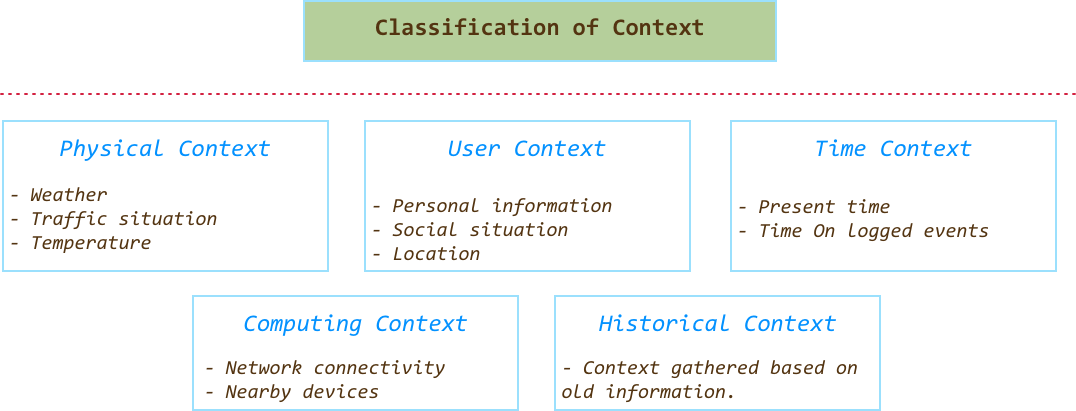
\includegraphics[width=120mm]{Classification_Of_Context.png}
  \caption[Classification of context.]{Classification of context information as per \cite{schilit1994context}}
 \label{figure:ContextClassification}
\end{figure}

Context Awareness on the other hand is the most basic building block for an anticipatory system. It specifies the ability of the system to know about the state in which it is presently in and eventually adapt itself to the conditions based on the knowledge it has gained over the period time about the user's choices. Context-awareness acts as an extension of human senses, fulfilling its limitation, helping in continuously understanding the user's context and improvising itself in its ability to help the user perform his tasks more effectively. Similarly as with all other computing problems, context awareness has moved far ahead from the initial description of context\cite{schilit1994disseminating} with the emergence of readily available powerful sensing devices in the hands of masses in the form of mobile smartphones hence allowing us to move ahead far more than one had imagined earlier.


\chapter{Ambient Intelligence \& Anticipatory System}

The field of ambient intelligence and anticipatory systems are closely interrelated with each other. Ambient intelligence acts as a foundation for systems which want to perform anticipatory tasks. Both can actually be considered as components of a system which Weiser might have envisioned when he said ``The most profound revolutions are not the ones trumpeted by pundits, but those that sneak in when we are not looking''\cite{weiser1991computer}.

The term \textit{Ambient Intelligence} was first introduced in the AmI Challenge in 2001 \cite{ducatel2001scenarios}, wherein it identified Ambient Intelligence at a conceptual level, highlighting the various components that would be required to make it a reality. \cite{sadri2011ambient} defines it as an environment wherein the the environment itself would adapt to the needs of the user, there would be a lack of any input device to take user's feedback instead there would be sensors which would blend in into the environment's day to day items, connected with each other and constantly trying to improvise and creating a positive impact in the life of the user.

Anticipatory system is described as ``a system containing a predictive model of itself and/or of its environment, which allows it to state at an instant in accord with the model's predictions pertaining to a later instant" \cite{rosen2012anticipatory}. Hence, the system has to be intelligent enough to make predictions about the future and also to adapt itself, this makes it very similar to ambient intelligence, the difference being that the ambience of the technology which allows it to render invisible to the user may or may not be there in the anticipatory system. The current framework and application mentioned further in this report form the ground work for a system which falls into the category of both ambient intelligence and anticipatory system.

\section{Components Of an anticipatory system}
An anticipatory system constitutes of multiple components which work in a synchronous manner to provide the desired end result to its users. As we have seen that the context for any action tells us a lot about the user, the action being performed and the reasons behind it, hence forming an essential part of any system that deals with understanding and improving user's day to day tasks and habits. Majority of the information required to do such a task is extracted from the sensors that are available on the devices, however the raw data has very limited use and usually bound to an individual. We require a larger dataset consisting of multiple individuals to attain the desirable results. After collection of raw data features are extracted from it and meaningful information is obtained helping us derive inferences. These inferences can then be used to predict future events and action, gradually improving itself and its ability to predict over a period of time in the form of reinforced learning. 
\cite{pejovic2013anticipatory} categorises the entire system into four staged process:

\begin{itemize}
\item Sensing of the contextual information
\item Extraction of features from the data
\item Making prediction based on the available data
\item Understanding its faults and improvising itself to provide more accurate and useful information
\end{itemize}

Let us further look into each of the above mentioned step in detail to understand how they function and fit together.

\subsection{Sensing}
First and foremost step in any anticipatory system is to collect information about its users. The information is in most cases, quasi-continuos sensor reading from the device's various sensors and various other sources of contextual data available for the user. The nature of data varies on various factors such as the availability of sensors, portability of the devices and the actual requirement of the system.

With the advent of modern mobile devices we have a plethora of sensors encompassed in a single portable handheld device which the user is almost certain to carry around and use continuously throughout the day. This presents an opportunity for us to extract meaningful information about the user in his natural environment without interrupting or obstructing his day to day task and definitely without him deviating from his natural flow of work. Almost every smartphone these days has basic sensors such a GPS. accelerometer, light sensors among other and can usually connect to the internet. This provides us with a very rich source of contextual information which we can harness for gathering data about the user. This is not just restricted to smartphones but can be extended to various other platforms such as music players (iPod), tablets (iPad, Nexus 10, etc.), gaming consoles (XBOX, Wii, Playstation), home theatre systems, vehicle GPS navigations and many other components that we interact with almost on a daily basis, all of which provide some source of context which we can put to use.

\begin{figure}[hbtp]
 \centering
 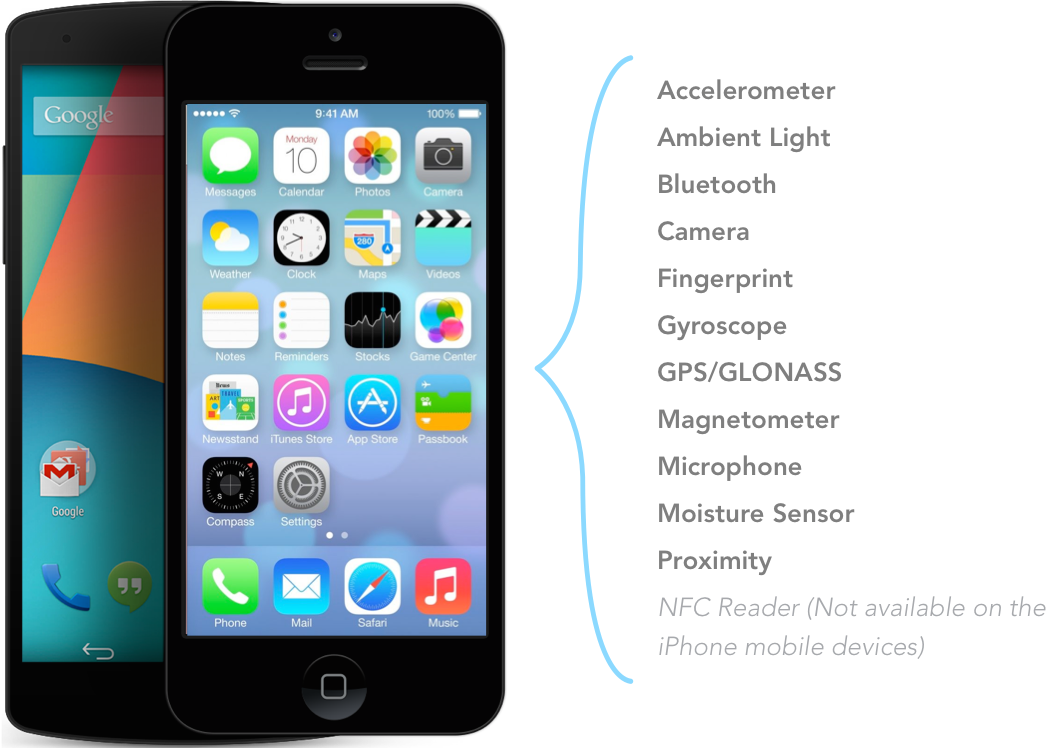
\includegraphics[width=120mm]{Sensor_List.png}
  \caption[Sensors on modern day smartphones.]{List of sensors that are available on modern day smartphones. \textit{(Apple iPhone 5S and LG Nexus 6 in the image)}.}
 \label{figure:SensorInformation}
\end{figure}

When we perform sensing on an individual and collect information it helps us in understanding an individual alone and is usually referred to as \textit{Personal Sensing} \cite{lane2010survey}. But with the recent growth in mobile internet networks, people are always connected and so are the devices to each other and to the web; this allows us to not only sense the information but also to store it onto a central location on the worldwide web. When sensing is performed on a larger scale i.e., where we are monitoring a group of individual or a certain community to identify patterns and emerging trends, this is termed as \textit{Crowd-sensing} wherein individual devices collectively provide data to identify trends which are of a collective value to the entire community \cite{ganti2011mobile}. There are already several real world examples which use community based sensing in areas like environmental monitoring \cite{dutta2009common} and navigation \cite{mohan2008nericell,hull2006cartel}. The only shortcoming of this technique is being unable to interact with the test users to take their feedback personally which is possible in the case of personal sensing.

Sensing even with all the vital information it provides is not without its owns issues and drawbacks. The availability of the data is very much platform dependent, with multiple devices and mobile operating systems, deployment is one of the key challenges along with the issues faced on each of the platforms. Additionally as it is with all areas of research which makes use of user's information, privacy of the user and of his information is a key concern. We will discuss this further in chapter \ref{challenges}.

\subsection{Feature extraction and context association}
The raw sensing data acquired from the sensors does not have much use, raw data contains a considerable amount of noise. We need to interpret the raw data to extract relevant features from it which is specific to the requirement of our application. For example we can have the raw data from the accelerometers but how do we understand from the accelerometer's x,y and z values the activity user is performing, if the user is currently travelling how do we infer the mode of transport. How do we decide if the user can be interrupted at any given point in time \cite{ho2005using}? There are various platforms and statistical tools readily available for analysing and deriving vital information from each of the raw data types. However each of the contextual raw data types can be used to extract various different characteristics \cite{pejovic2013anticipatory}. For example sound can be used to identify the present surroundings of the user however it can also be used to understand the physiological state of the user as well \cite{lu2012stresssense}. So the feature extraction actually depends on what is the required end product and whats the role of the contextual information in making the end product a reality.

Additionally, there are other co-context's that can be fetched using the available contextual information. For example, having location of the place where the user would be in the next few hours enables us to fetch weather forecasts for that area, hence weather becomes a co-context. Similarly, if location itself is not directly available but we have cell tower information or WiFi information we can calculate the location from based on it.

\subsection{Anticipation, improvement and self-learning}
Understanding the features and extracting the information from the raw provides us with an opportunity to use this information for much more then understanding the present context of the user. By knowing what user's choices are we can make predictions for the future. For example, let us consider an example application which monitors location and accelerometer data using the user's mobile device. After a period of time through feature extraction the application would develop a user model according to which the user travels everyday at 9am to his office and uses the train as the means of transport. The application can then predict his travel schedule and provide train timings in the morning before he leaves his home. Additionally it can also notify the user if he is late by identifying deviation from his daily behaviour pattern.

From the extracted features various supervised learning models can be constructed which can associate user's activities and the related context. For example, in the travel prediction application, we can verify the user did take the train specified by the application or not based on which we can strengthen our prediction model. This when applied to the collective data of the community helps us build an effective model which can help us anticipate things which would be useful for any user in that community.

\section{\textit{WebSense} as an anticipatory system}

\textit{WebSense} along with the context sensing framework lays a foundation for various viable anticipatory system, even at present it partially fulfils role of an anticipatory system in the form of \textit{WebSense}. To understand how the system works as an anticipatory systems we need to understand the various components which interact with each other and other components that can be linked with it to make it a complete anticipatory system.

The primary component of the system is to gather information for further processing. This task is performed using the context sensing framework, which provides all the context information based on subscriptions. Other then context, user's application usage is also one of the most vital component of the system. This is extracted from the mobile's default API. The framework and the sensing process and strategies are explained in further detail in chapters \ref{ContextSensingFramework} and \ref{DemographicsApp}.

Since the application falls in the category of crowd-sensing, the data is sent to a central data store on the web from the various devices of individuals. The application makes sure that the data is sent to the server in a power and money efficient manner. The server is responsible for storing the information securely and also acts as an authentication server. Essential features are filtered and context is associate with each other and the user. Further also tries to understand the extracted information and provide end points for the application to get prediction data and analytics information (See chapter \ref{DemographicsApp}).

As you will see in details in the chapters ahead, the application takes into consideration each of the aspect of the anticipatory system. There is much room for improvement in all of the components especially predication and self improving mechanism which will be further discussed in chapter \ref{futureUser}.


\chapter{Android Context Sensing Framework}
\label{ContextSensingFramework}
Context is a very primal component in all of the anticipatory systems. As one can conclude from figure \ref{figure:SensorInformation}, the contextual information that can be gathered using modern smartphones is a lot and more and more sensors are being added onto the devices with every new release. However, there are various mobile platforms and each consisting of its own development environment, tools and deployment stores making it very difficult to develop a framework which can function on multiple platforms. For the purpose of this project selected the Android development environment for various reasons. The platform this provides a much more flexible and open framework to extract contextual information. It also the most widely used mobile operating system and consists of devices of all price ranges hence providing a much more diverse target audience.

Although there have been many contextual frameworks in the past some of which are for Android as well; providing a relatively easy methodology to extract meaningful information \cite{novakextensible2013,rachuri2010emotionsense}, however the present requirement of the project is much simpler and there are some components that the frameworks presently do not monitor, for example, \cite{novakextensible2013} does not monitor network, WiFi access points, \cite{rachuri2010emotionsense} does not monitor user's schedule and phone profile. Also a framework at this point would provide more flexibility and access to the more recent API's which older frameworks do not cover. Although The context sensing framework designed for the purpose of this project but it is designed in a way to interface and connect to any application for monitoring purpose.

\section{Contextual information types}
\label{contextType}
There are various sensors that are available for the purpose of monitoring in the modern mobile devices and supported by the Android SDK. The following are the contextual information which were considered to be supported and available for subscription in the first version of the framework.

\begin{itemize}
\item Location (GPS or Network)
\item Battery/Power source information
\item Network connectivity status
\item Network signals (Cell tower connectivity)
\item WiFi access points and connectivity status
\item User events
\item Bluetooth status and nearby devices
\item Telephony events
\item Screen activity context
\item User phone profile (Screen brightness, Volume settings \& Vibration)
\end{itemize}

We will further discuss a few of the the above mentioned context's in details and how a scanning methodology was customised for it be both effective and efficient.
 
\section{Framework's working architecture}

In order to understand how the framework would actually function once integrated we divide the system's architecture into two components, first is the external end points of the framework which any application can interact with the second component is the actual internal component which handles subscriptions, monitoring, polling and content delivery.

\subsection{End-points and external handling}
\label{ExternalHandling}

As we described earlier the purpose of creating a new framework is to make sure information is provided in the simplest possible way and should be extensible. Also the framework has to be plug and play, there should be very minimal code that would have to be written on order to integrate it with an existing application and to perform what is required. The functionality of any existing application should not turn away from its original goal to focus on the integration of the framework and procuring data from it. The framework should just be a component integrated into the application providing a stream of required information and which can be controlled by the application.

The framework's architecture can be described as a subscription based model, wherein each of the components can be subscribed externally by the connecting application. In addition to that each subscription can be provided with additional parameters in order to tailor the subscription based on the needs of the application.

To begin monitoring any particular context one just has to call the \textit{monitorContext} method from \textit{ContextManager} object. The call then initiates a monitoring service for the context based the parameters that is being passed along with it.

\begin{program}
  \begin{verbatim}

public void monitorContext (
            ContextManagerServices mService,
            long minimumUpdateTime,
            long pollingTime,
            ArrayList<Integer> flags
    );
\end{verbatim}
\label{monitorContextCall}
\caption{Function definition of the monitor context.}
\end{program}

As we can see in the function call, there are several parameters, let us look into them for more detailed understanding of the function's actual functioning.

\begin{itemize}
\item \textbf{\textit{ContextManagerServices} Parameter - } \textit{ContextManagerServices} is an enumeration defining various types of contexts that can be monitored by the framework, this specifies which context the application wants to monitor using the framework.

\item \textbf{\textit{minimumUpdateTime} Parameter - } This specifies the minimum time the application should wait before sending a forced broadcast about the context regardless if there is any change in the context or not. This is useful for application which want information about context at regular intervals regardless of the magnitude of the change.

\item \textbf{\textit{pollingTime} Parameter - } This parameter specifies the time interval after which the framework should poll the sensors or the operating system for information about the context. This is specifically for information which do not have system provided callbacks (Broadcast/Intent architecture) and require polling or in cases where power consumption for constant monitoring is too steep and is not feasible (e.g. GPS based location monitoring).

\item \textbf{\textit{flags} Parameter - } This is an extensible parameter which is essentially an array of flags which can be passed to the framework. This also provides a backward compatible way to extend the framework without changing the original function call definition. An example for the use of this parameter is for passing information about the source to use for location tracking to use while performing the polling task.

\end{itemize}

With the help of this single call, one could start monitoring any contextual information that is made available in the present version of the framework. In case of missing parameter related to the timing information, the framework uses a constant value for monitoring tasks which is customised for differently for each type of context.

\begin{figure}[hbtp]
 \centering
 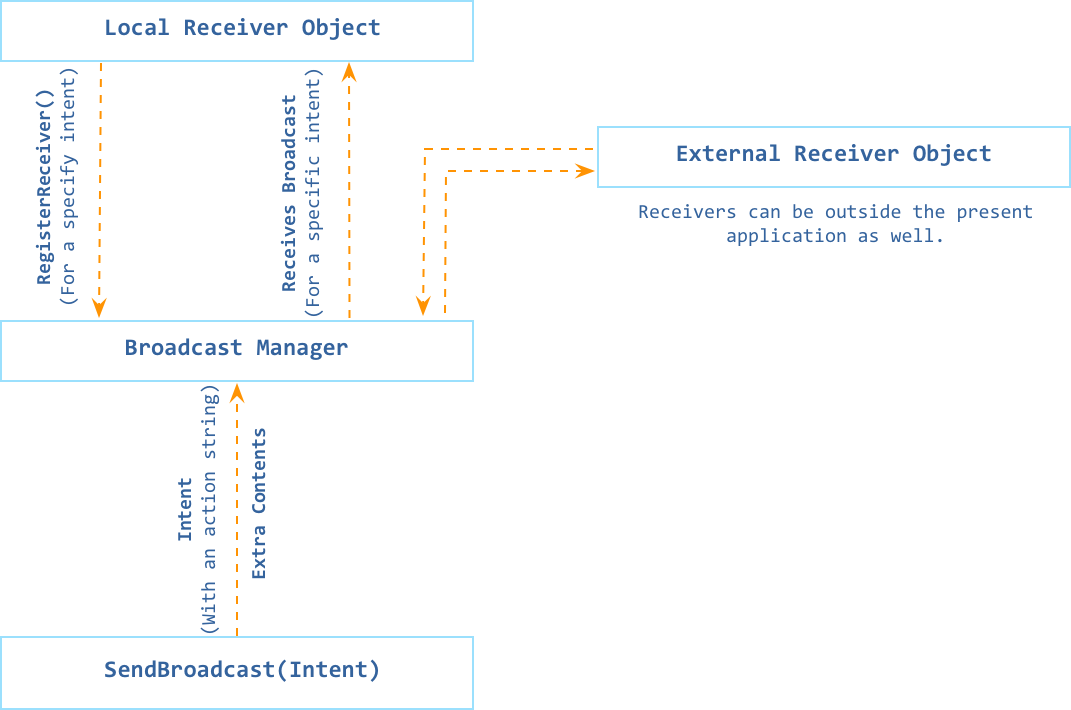
\includegraphics[width=130mm]{BroadcastReceiverModel.png}
  \caption[Architecture for the information broadcasting model.]{Architecture for the information broadcasting model.}
 \label{figure:BroadcastRecevierModel}
\end{figure}

To notify the application about contextual information the Android platform provides a very effective methodology to transfer information between the framework with the help of \textit{BroadcastManager} which sends a message called \textit{Broadcast} to all the \textit{BroadcastReceiver}. The working of the methodology is very simple yet very effective. As figure \ref{figure:BroadcastRecevierModel} explains we can ask for an object to register itself to the \textit{LocalBroadcastManager} to be notified in case it receives a broadcast with a particular name or tag which is referred to as \textit{action} in Android.

The framework uses the same action string for all the notifications with more detailed information about the content being supplied inside the \textit{Intent Bundle}.


\begin{figure}[hbtp]
 \centering
 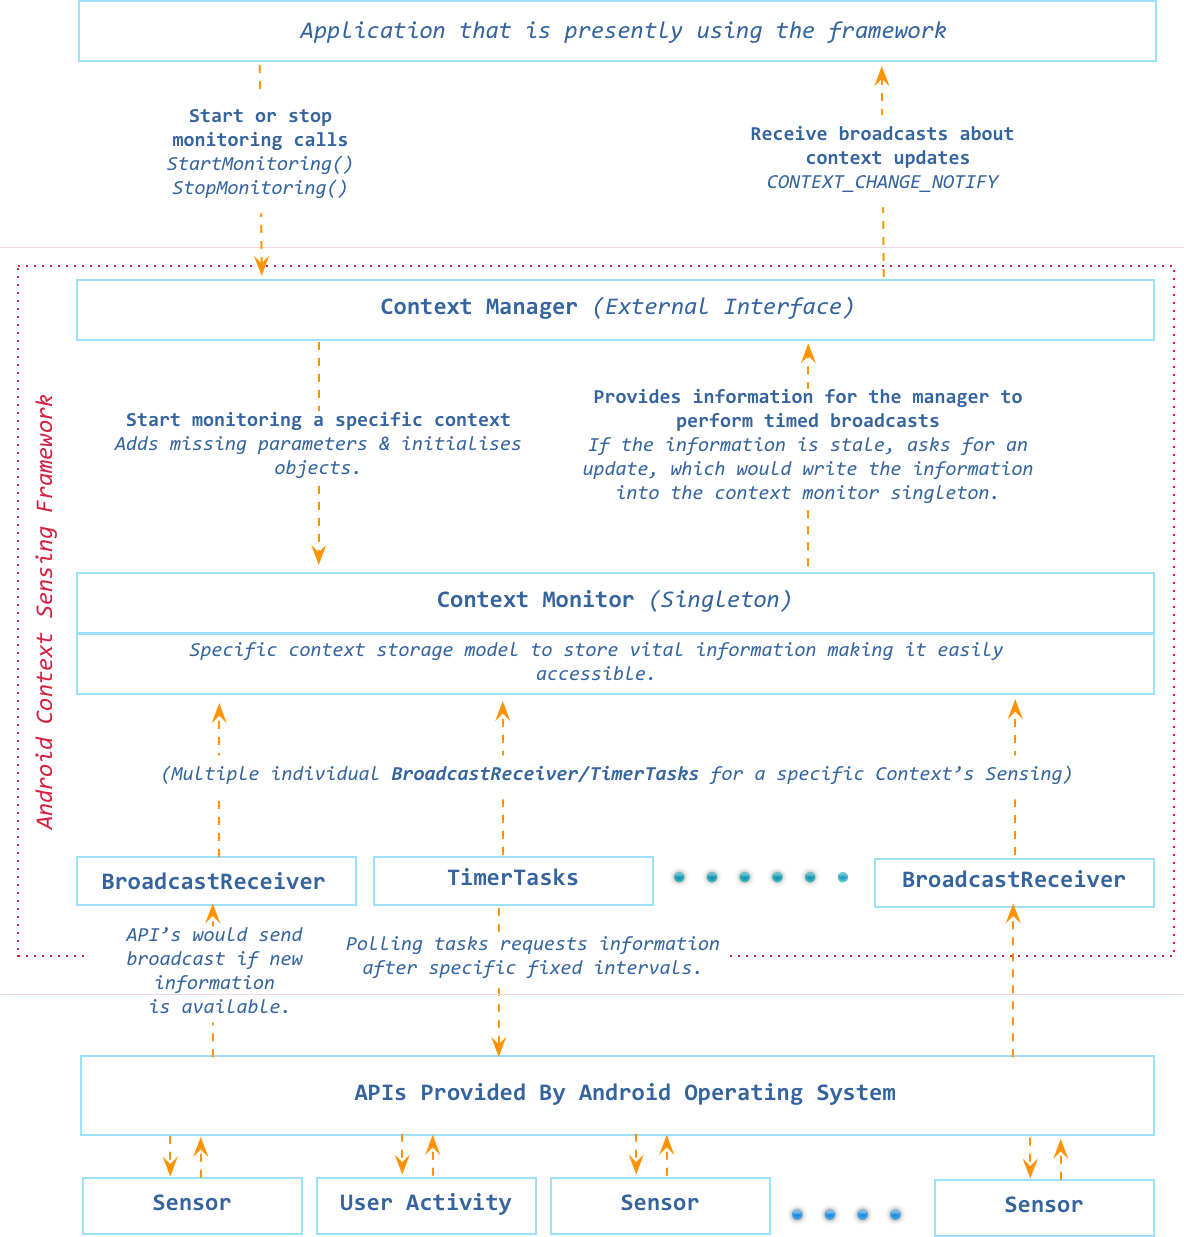
\includegraphics[width=150mm]{FrameworkArch.png}
  \caption[Architecture of the Context Sensing Framework.]{Architecture of the Context Sensing Framework.}
 \label{figure:FrameworkArchModel}
\end{figure}

The application using the framework would have to register a broadcast receiver just once to the\textit{LocalBroadcastManager} for any and all contexts the framework is monitoring. When the framework has an update it would send a broadcast consisting of the following components:

\begin{itemize}
\item \textbf{Action - } All broadcasts from the application are associated with one action string `\textit{\textbf{CONTEXT\_CHANGE\_NOTIFY}}' regardless what type of context it is.

\item \textbf{Additional Information - } Other then the action string, broadcast also contains additional information in the form of a collection of key/value pairs. The framework sends various other values along with each of the broadcasts.
    \begin{itemize}
    \item \textit{\textbf{CONTEXT\_TYPE - }}The type of context the broadcast contains.
    \item \textit{\textbf{Context Information Flag - }}This information is passed with the key named after the context type that is passed, hence varies depending on the content it contains. The value is a JSON (\textit{JavaScript Object Notation}) formatted string containing information passed by the framework.
    \end{itemize}
\end{itemize}

Finally, the application should be able to stop monitoring a context as easily as it begin monitoring the context. The context can be stopped from being monitored and hence the application would receive no further updates by simply calling

\begin{program}
  \begin{verbatim}

public void stopMonitoringContext(
            ContextManagerServices mService
        );
\end{verbatim}
\label{monitorContextStopCall}
\caption{Function definition to stop monitor context.}
\end{program}

\subsection{Internal working}

The internal working of the framework constitutes on multiple components of the framework working in parallel and interacting with each other constantly. As described in section \ref{ExternalHandling}, \textit{ContextManager} is the external interface with which applications trying to use the framework would have to interact with. The class is also responsible for delivering broadcast at specified \textit{minimumUpdateTime} interval. However, the framework is build on a on a set of classes which ensure that latest information is always made available to \textit{ContextManager} and is done is an efficient way.

A singleton class, \textit{ContextMonitor} is primarily responsible for performing all the monitoring tasks at the specified time intervals and updating the values for the \textit{ContextManager} to access and pass on further to the application. There are two kinds of context extraction process that the class has to deal with.

\begin{itemize}
\item \textbf{Monitoring Tasks - } Certain contexts have a broadcast and intent model provided by the operating system, in which case, a broadcast receiver for that specific action string is created in the singleton to receive information and update its variables accordingly and in case of a relevant change a broadcast is sent to the receivers. The subscription to receive the update is added and removed whenever the applications requests the framework to.

\item \textbf{Polling Tasks - } Certain contexts need to be accessed using Android system API. These calls would have to be made at the specified time intervals to keep the information updated. For this purpose we use a timer task in \textit{ContextMonitor} and is triggered when monitoring is requested. In case there is a relevant update in the information a broadcast is sent to all listeners about it.

There are several advantages of using this development model, primarily this provides a single point of access to all the information that is required by the framework which provides easy of use and extensibility to the framework. Additionally, a single instance of the monitoring task ensures there are no multiple tasks being run by the framework for the same type of context which can be accidentally triggered in case the application using the framework starts to monitor same context at multiple places if the singleton was not in place. Although the framework provides a very resource effect method to gather information (see \ref{PeformanceEval} for performance benchmark).
\end{itemize}


\section{Understanding individual context monitoring}
Each of the context's being monitored by framework have their own unique methodology in which they work. The uniqueness helps them to perform monitoring in a very effective and power efficient way. Let us look in details a two of the important context's working.

\subsection{Location}
Location is one of the most important contextual information that can be extracted by the framework. With modern devices which people carry everywhere it has become all the more important. The major concern with location monitoring is the power consumption factor when using GPS \cite{ben2009less}, so continuously monitoring of GPS is never recommended on mobile devices. Also, time it requires to switch on the GPS sensor. Getting a triangulation from the satellites can also be a time consuming task sometimes. Modern devices provide network based location services which require both network connectivity and internet to provide location. This process is battery efficient but accuracy is usually questionable. 

The framework provides the application option to opt for either of the technique in addition to the ability to specify the polling interval.

\begin{figure}[hbtp]
 \centering
 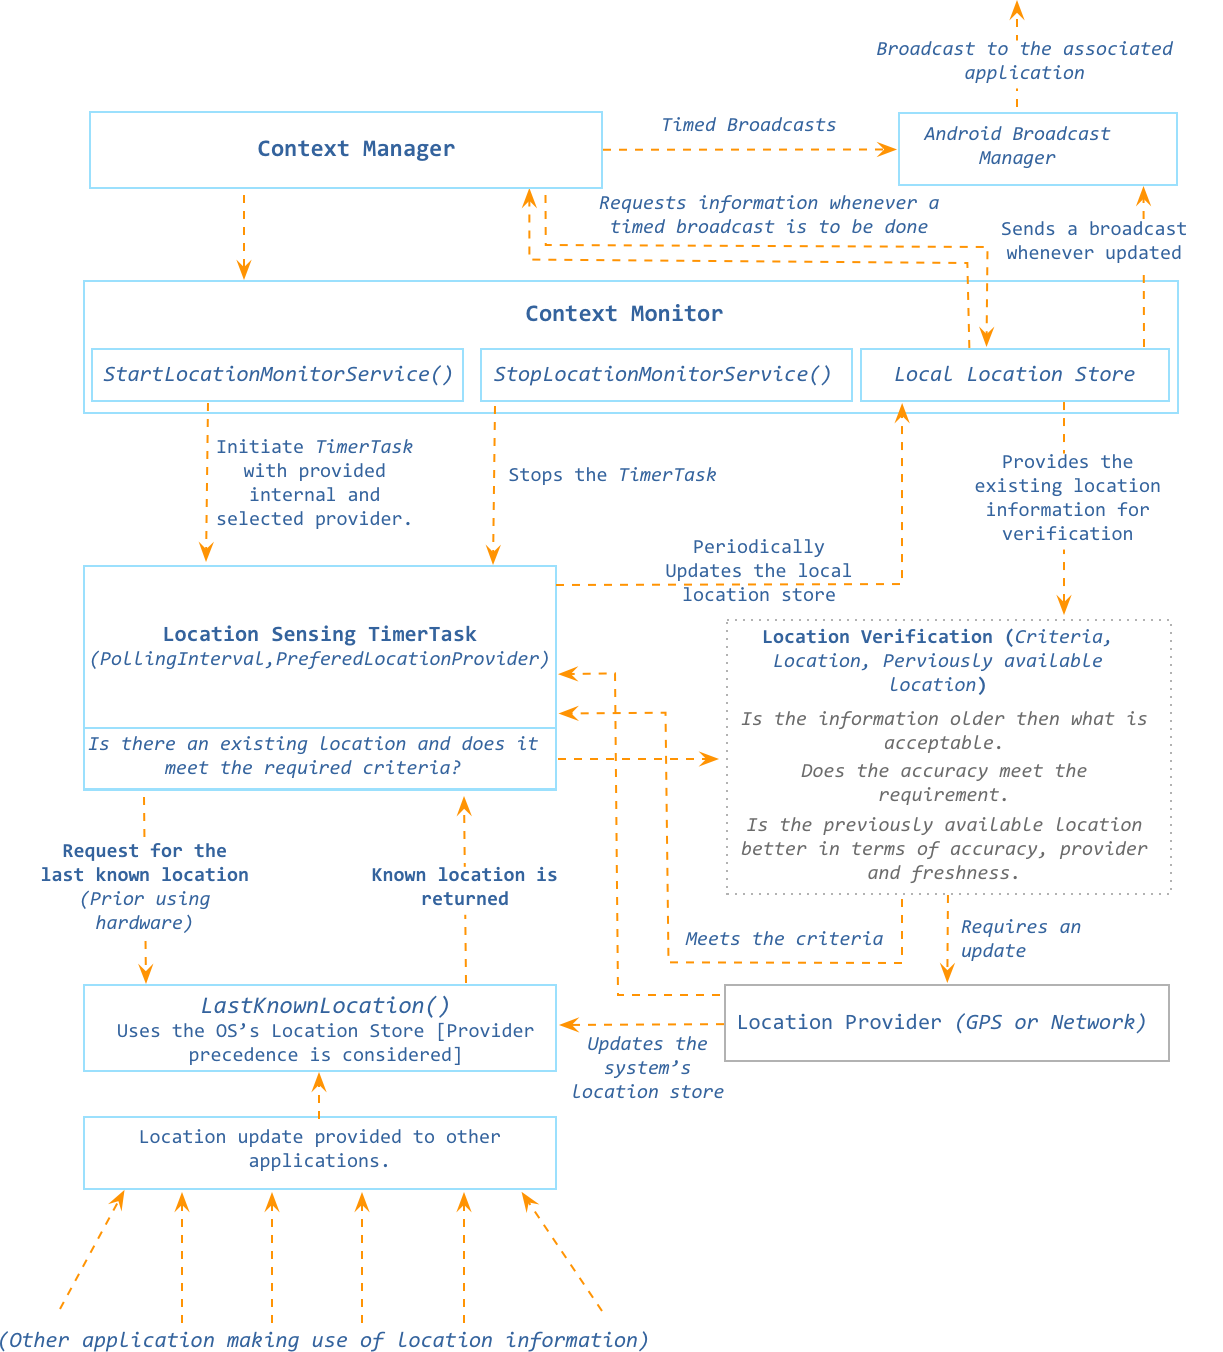
\includegraphics[width=160mm]{LocationSystemArch.png}
  \caption[Process for efficient monitoring of location.]{Process for efficient monitoring of location.}
 \label{figure:LocSysModel}
\end{figure}

Android operating system stores the last known position\footnote{http://developer.android.com/reference/android/location/LocationManager.html\#getLastKnownLocation} which is updated when any of the application tries to fetch location using GPS or network provider. So once every few minutes (defined by the provided polling time) the device first looks for location that is stored using the \textit{getLastKnownLocation} method. Then the framework analyses if the location that is being provided by the system is a better location then the one it already has and if it meets the criteria (see figure \ref{figure:LocSysModel}), if the criteria is met this location is stored and broadcasted. If not, the system would trigger the specified location provider (GPS or Network) to provide it with a new location, the fetched location is then broadcasted and stored.

\subsection{Network information}
Mobile phones are almost always connected to a cellular network, when the user moves the network connection also changes. The systems decides which of the towers providing signal to connect to out of the various ones that are available. This information can be very useful in terms of context. For example with this information one can map the network density and signal strength of the area. There are several components that constitute of network information and there is not a single method to monitor this.

\begin{itemize}
\item \textbf{Signal Strength - } Signal Strength constantly changes and can be monitored by a system provided broadcast receiver. However the frequency of the change is very high, hence broadcast is done only when there is a significant change in the signal levels.

\item \textbf{Cell Towers Nearby - } Although the device usually connects to a single cell tower but there are various other towers which broadcast their presence and the device picks it up along with other information such as their signal strength. This information is also provided through a broadcast receiver by the system.

\item \textbf{Data Connectivity - } The networks may or may not be providing data connectivity to the device or the user might have turned off the data connectivity. This information needs to be polled constantly as the broadcasts are not reliable and do not provide internet connectivity information. The framework frequently checks for updates about connectivity information and notifies if there is any change.

\end{itemize}

\section{Shortcomings and possible improvements}
\label{contextShortcomings}
The framework provides a solid foundation with features that make it extensible and might provide useful to various kinds of application and research work on the Android platforms. There are several areas which should can be optimised and improved further in the future versions.

Firstly, the framework can be made more robust and reliable. Currently it has been designed for devices running Android version 4.0 and 4.4, backward compatibility would certainly make the framework useable on a wide range of devices providing more diversity to future studies. 

Although android is at present one of the most popular operating system in the mobile market, there are a considerable number of the mobile users who use other popular operating systems like iOS and Windows platform, an extension of the sensing framework with similar functionality (within the bounds of the operating system) on other platforms would be certainly helpful in conducting studies with a broader group of audience then just people using android.

Additional context's like accelerometer, proximity, ambient light and application monitoring (currently implemented in an external build over the framework) are presently missing in the framework and would be valuable additions to it.

The sensor information gathering technique is very basic in nature and lacks adaptive qualities like in more complex libraries EmotionSense \cite{rachuri2010emotionsense}, which allows the sensing to be done in an adaptive manner instead on a fixed interval. For example movement of the user should be tracked based on the movement he has done during the previous time interval, if the location change between two interval is considerably less or none at all, the next sensing should take place an increased time interval then usual or if the change is considerable the sensing time interval should be reduced. Additionally, it should take into consideration the battery usage of the sensor and the current state of the device, i.e. sensing intervals should adapt itself based on the battery life of the device to improve overall performance of the framework.

Given enough time the framework can be expanded into a much more robust, functionally rich and highly customisable component which can be used in various kinds of studies and real world application.

\chapter{User's smartphone usage data collection application}
\label{DemographicsApp}
The most essential goal of this project is to devise a technique to gather information about how a real world user interacts with his mobile device on a day to day basis in his natural and unmoderated environment. The context sensing framework provides a very robust foundation using which we can gather information about the context in which the user is using the mobile device. But at present the framework does not consist of any possible way to monitor and gather information about mobile phone interaction of the user both in terms of web and application usage.

\textit{WebSense} is an application for the Android platform developed for the very purpose of collection of user application usage data collection along with the related contextual information. The application is integrated with the context sensing framework described in chapter \ref{ContextSensingFramework} which it uses to extract contextual information of the user.

There were two aspects of the application which were taken into consideration while designing the architecture of the application. First was the actual development of the monitoring functionality to provide an efficient way that was to be used to monitor how the user interacts with the device in a ubiquitous way and eventually send it to a central data repository on the web for collective analysis. Second aspect was the utility value it should provide to the user which is essential for crowd-sensing application as apps in the crowd-sensing domain should be lucrative enough for people to install even if they are not interested in the research value of the application (see section \ref{PlatformDeployment} for deployment challenges). In the following sections we look into each of the aspects and the various components which collectively provide a skeletal over which the application functions.

\section{Application usage demographics collection}

Android is a very open platform in terms of providing access to data sources when we compare it with the other most popular operating system for mobile platforms such as Apple's iOS \cite{AppleiOSPolicy}. This allows us to develop application which can monitor user interaction in detail.

The most essential criteria of any monitoring application is to maintain a near 100\% uptime, which means that the app should always be running in the background and performing the necessary operations. Implementing a front end interface provides user an option to terminate the process very easily by accident or intent hence denying the change of gather information. However a background service on the other hand is more complicated to be terminated and also ensures that no hinderance is caused to the user in performing his day to day mobile phone usage. Hence the architecture of the app consists of several of background services each with their own set of responsibilities. This, along with a design to ensure that the monitoring service is switched on in case of device restart, accidental termination by the operating system or in case of an internal malfunction causing the termination of the application provides the system to operate at a near 100\% uptime (see chapter \ref{PeformanceEval} for detailed evaluation).

\begin{figure}[hbtp]
 \centering
 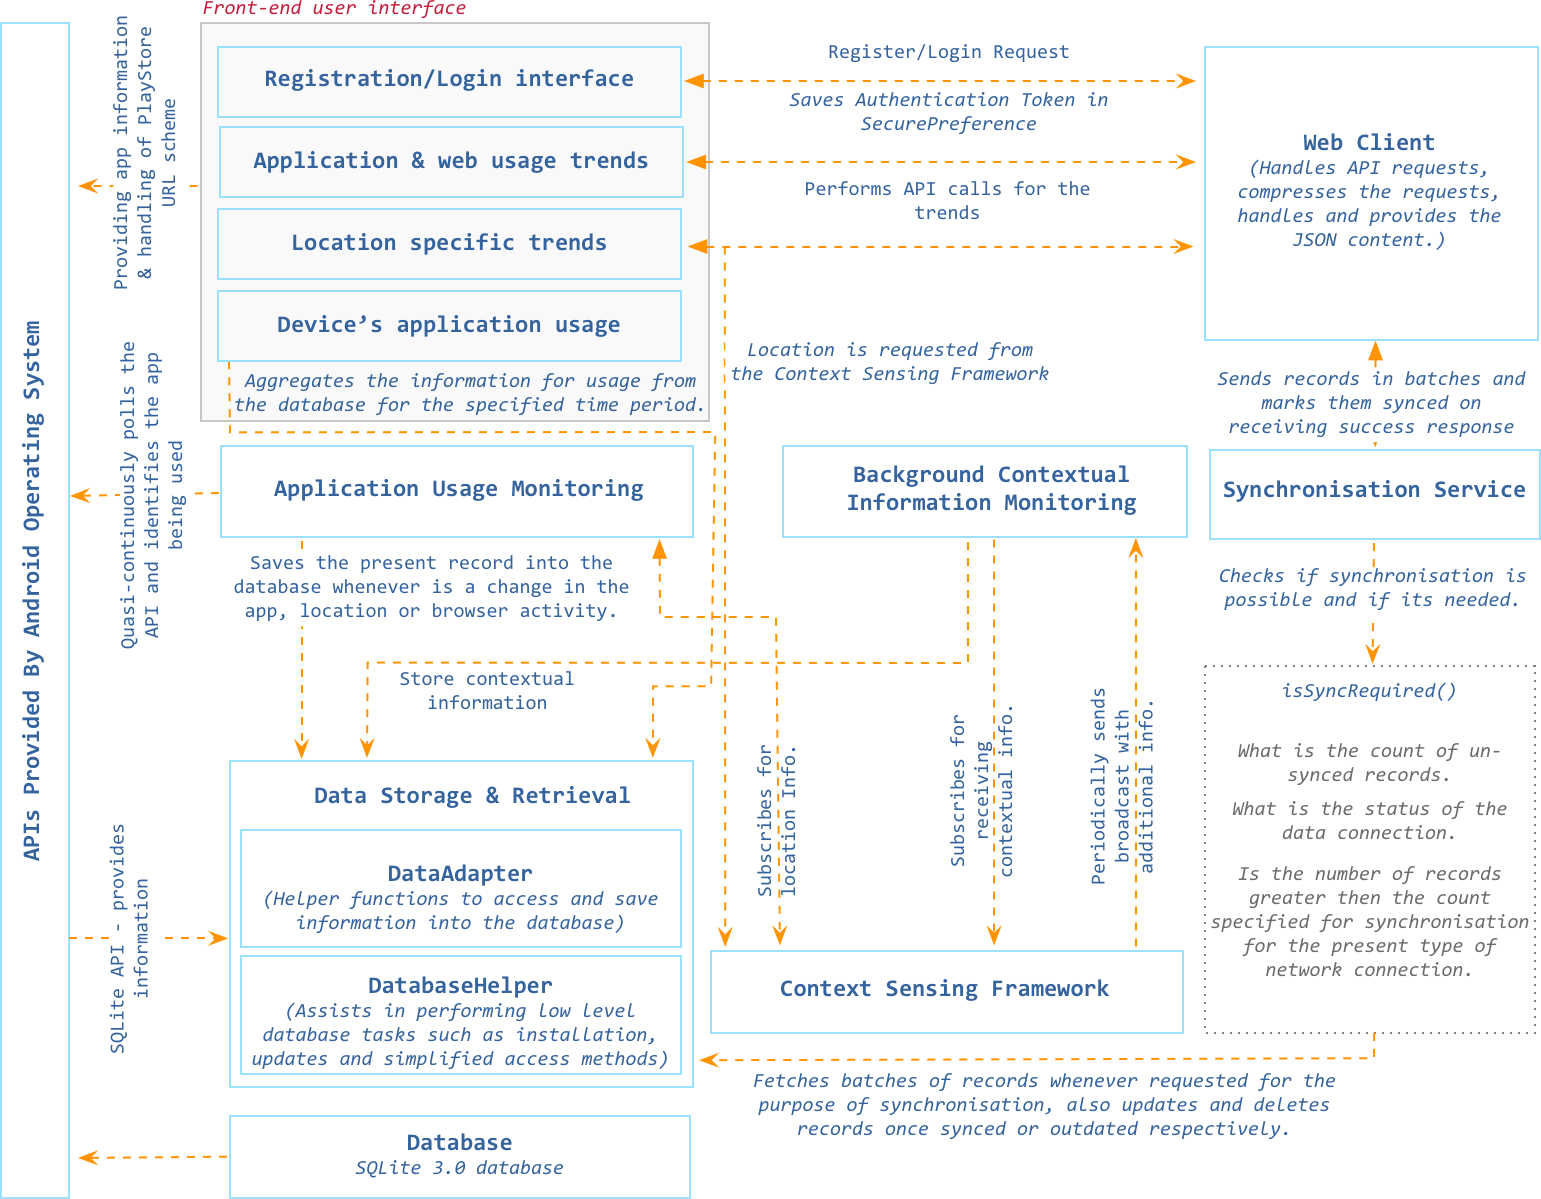
\includegraphics[width=160mm]{WebsenseArch.png}
  \caption[Architecture of \textit{WebSense} Android Application.]{Architecture of \textit{WebSense} Android Application.}
 \label{figure:WebSenseArch}
\end{figure}

Let us look into the various background services along with their role in the overall architecture of the system.
 
\subsection{Application usage monitor}

The primal responsibility of the app is to monitor the user's application usage continuously and with certain level of dependability. This task is performed by the service \textit{AppUsageMonitor}. The service is a self-reviving service so in case it is terminated either by the operating system or due to a malfunction it revives itself within a matter of seconds, ensuring an almost 100\% uptime.

Since Android does not provide a broadcast or any sort of delegation methodology to know when the application is switched, the only possible approach to do this at present is a quasi-continuous monitoring of the device's application stack. An interval of 4-second was chosen between each scan since research has indicated that user's attention span switches between the device and the environment somewhere within this duration \cite{oulasvirta2005interaction}, hence we can assume that the user would switch applications as well at around the same frequency. Android provides access to the list of currently active processes through the \textit{ActivityManager} class. The class not only provides information about the running tasks but also provides a mechanism to access the order of the application's screen presence. With this information we can identify which application is currently running and being interacted with on the device by the user.

Android also equips its developers with intents which one can listen to for detecting user's action of turning the device's screen on and off. This allows us to stop monitoring user's activity tasks when the phone is turned off hence saving crucial resources.

The application uses SQLite database\footnote{ self-contained, transactional SQL database engine — https://sqlite.org/} to store the monitoring information. This includes package name of the application, start time, end time (Both in UTC timestamp format), duration of the run, location it was used at (subscribes to the framework, listens and stores location information constantly) along with the day of the hour the application was used at. Additionally, a flag marking the synchronisation state of the record is also maintained. 

Whenever an application switch is performed the data is written into the database hence minimising the chances of data lose incase of a malfunction or termination. The information is also saved in the scenario when location update is received while an application is running, hence splitting a continuous session of the application based on the location. This is particularly useful in case of navigational applications as the user would keep it open over an extended period of time while his location changes constantly.

If the application is detected to be the default browser of the device, the app also gathers information about the page user is presently viewing. Although, there is no direct way to perform this, android provides an API to access browser history\footnote{Browser Data Provider - http://developer.android.com/reference/android/provider/Browser.html}, the most recent record in history would be the page the user is viewing currently. Whenever user changes the URL a new record is created and hence the time spent on a particular URL is also recorded.

\subsection{Contextual information monitoring}
\textit{ContextBackgroundMonitor} class is also a background service which is responsible for registering and monitoring the contextual information. Presently it monitors all the contextual data provided by the framework (see section \ref{contextType}). It is responsible is to make sure that as soon as the service is initiated it subscribes to all the available contextual information provider and whenever there is any new information made available by the framework it saves it in the database. Since we require information about location for mapping the information geographically and also have to provide user with information in relation to his location, all the context information is stored along with the latest location information attached to it.

The class is initiated as soon as the monitoring begins and when the class is destroyed it releases all the receivers and initiates the stop procedure in the framework (see section \ref{ExternalHandling}) hence stopping monitoring process altogether.

\subsection{Web synchronisation service}
The context sensing and the application usage monitoring generates a considerable amount content in terms of memory. This can directly be used for the purposes of local mining (see section \ref{AppUsageInfo}) but this being a crowd-sensing application, we need the information at a central location to further analyse information of the user-base as a collective. For this purpose, the information that is in the local datastore has to be constantly sent to the remote server on the web.

The class \textit{SyncManager} performs all of the synchronisation of the device with the web by uploading the information in the most efficient way possible. After a certain interval of time the class triggers a method to check for a possibility for a need of uploading of the information. Records which have not been synced in the database is the first criteria the method checks for. To avoid repetitive reads to count un-synced records the monitoring services automatically increments the count whenever a new record is added and stores it on a preference file, this file is read by the synchronisation process. If the criteria for data upload is met the information is uploaded in chunks of fixed number of records in the form of a JSON string and once the data is successfully uploaded the records that were sent are marked as synced. The synchronising process uses the end points provided by the web application and sends the data after compressing it using GZIP \footnote{GZIP File format specification -http://tools.ietf.org/html/rfc1952}. The records are sent with an authentication key to both validate and associate the records, this key is obtained during the login process (see section \ref{LoginInterface} and \ref{StoringInfo}).

The service is also responsible for periodically clearing old data which has been synced already and are beyond the time-period which is relevant to the application (30 days in this case).

\section{User interface \& Providing utility value to the user}

The monitoring and reporting aspect of the project could have been done without actually a front end with everything entirely handled by background services but the primary test subjects of this application are not a selective group of people, like any crowd-sensing application the future research based on this application tends to make this available to as many users as possible, not only the people who are interested in the research aspect but common public with Android devices. As we will see later on in chapter \ref{challenges} one of main issue when dealing with crowd-sensing application is that it is bottle-necked by the fact that the entire research, application's widespread usage and the amount of data gathered depends solely on the decision of the user to install and keep the application on his phone. So to ensure widespread participation and retention of the application we need to provide the user utility value through the frond end of the application, so regardless if the user is concerned with the study or not he would still have a reason to install the application.

The user interface of the application which runs atop the data gathering services provides 
Information and feedback to the user and also helps in gathering certain user's personal information. The application is also integrated with a crash reporting framework called ACRA \footnote{Application Crash report for Android - https://github.com/ACRA/acra/} which provides the crashes and issues faced by the users to the web server, helping us to improve the application's performance and making it more stable.

\subsection{Login/Registration interface}
\label{LoginInterface}

\begin{figure}[htbp]
 \centering
 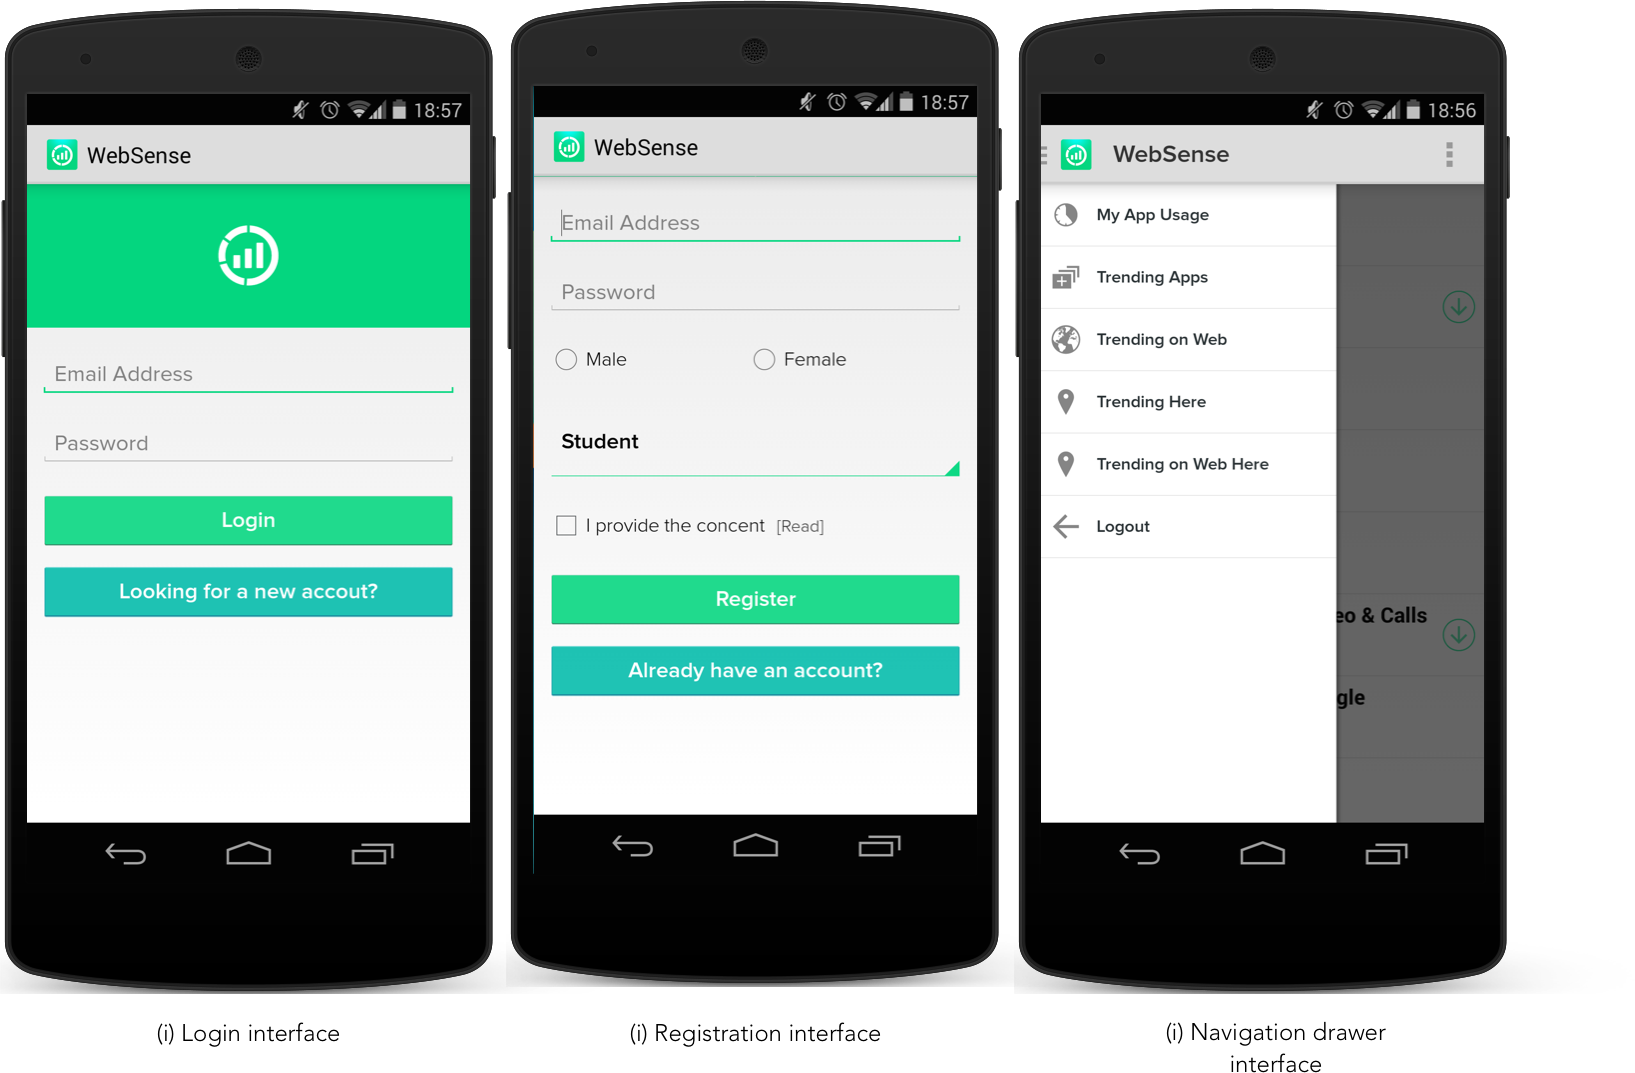
\includegraphics[width=150mm]{AppInitialScreen.png}
  \caption[Initial screens of \textit{WebSense} app.]{Initial screens of \textit{WebSense} app related to authentication and basic navigation}
 \label{figure:SensorInformation}
\end{figure}

The login/registration interface is the initial screen of the application where in the user provides the below mentioned information if he is registering or just logs into the application if he has already registered.

\begin{itemize}
\item Email Address - Allows us to have the means to contact the user in the future.
\item Password - For authentication purposes in case the user logs out or wants to login on another device.
\item Gender - Can be used as a metric to perform future studies.
\item Employment Status - Additional parameter which can be used in future studies.
\item Consent to allow monitoring - Along with a link to the End user's license agreement.
\end{itemize}


The application allows multiple sessions using the same credentials on multiple devices. An option to log out of the application is also provided inside the application, in case the user wants to do something privately or wants to stop monitoring completely.

\subsection{Application usage information}
\label{AppUsageInfo}

\begin{figure}[htbp]
 \centering
 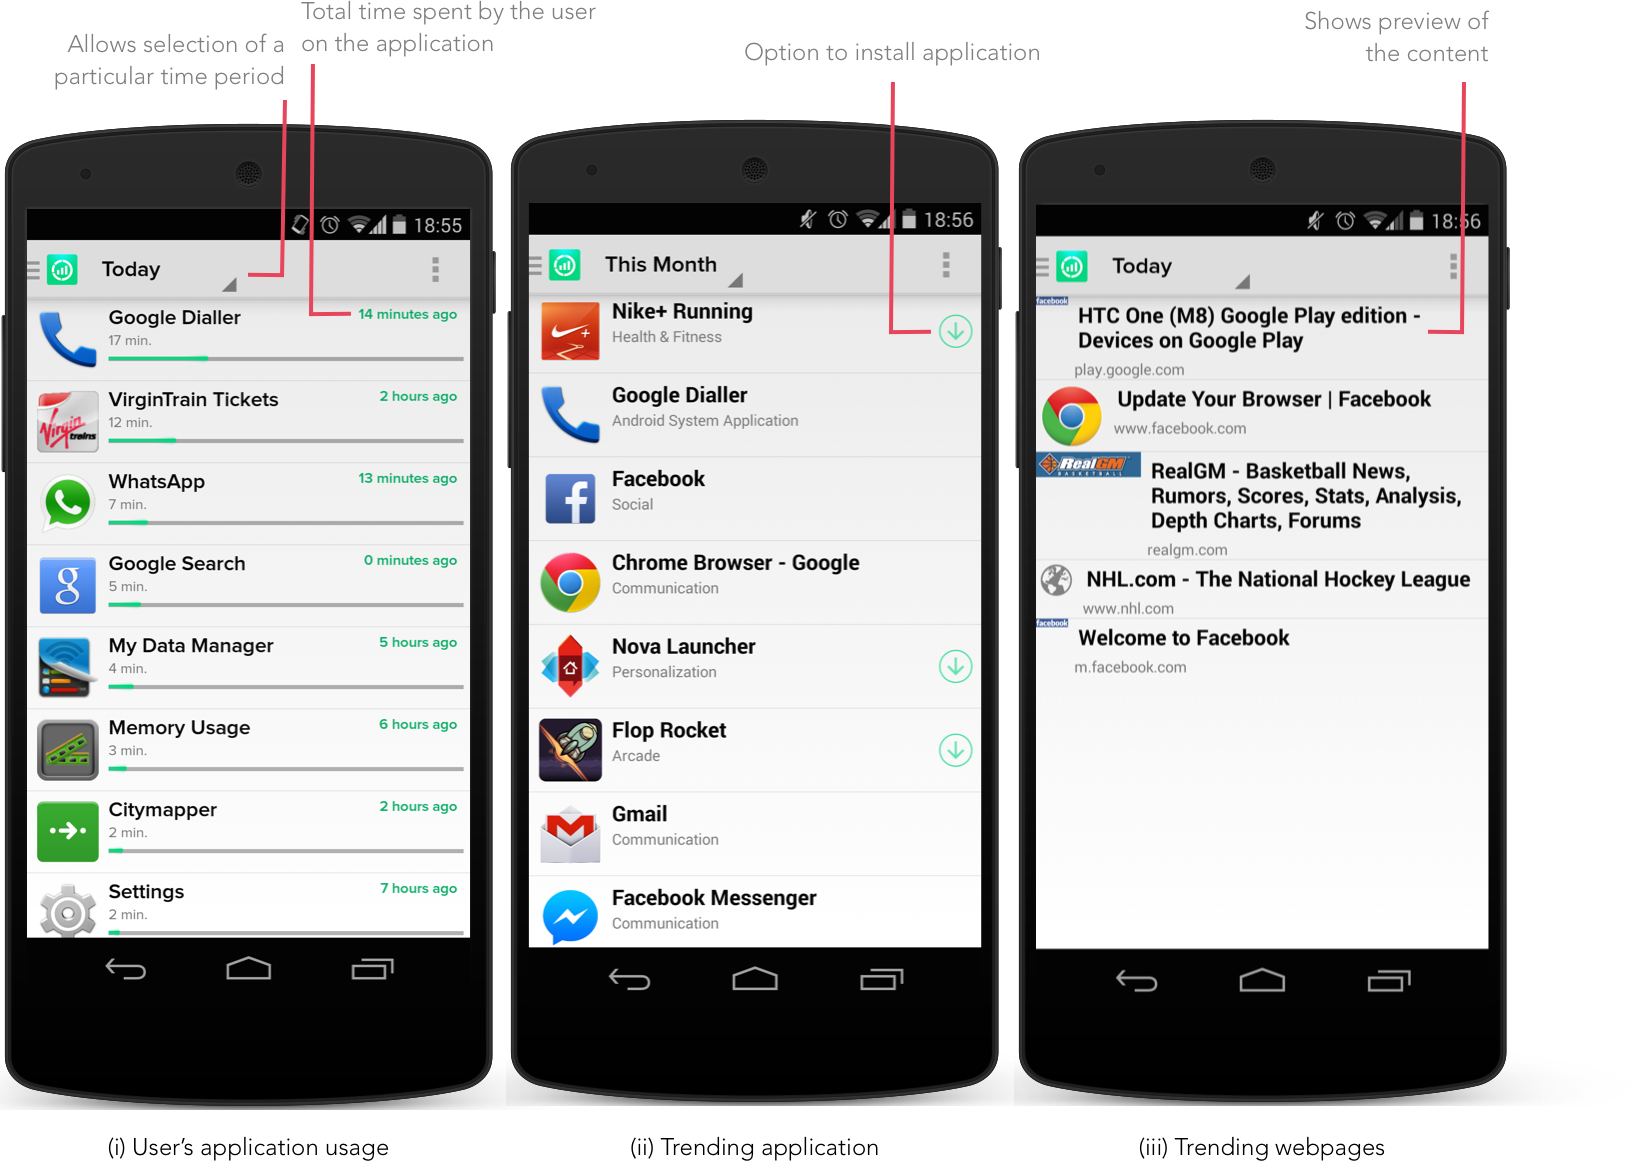
\includegraphics[width=150mm]{AppListScreen.png}
  \caption[Content display screens of \textit{WebSense} app.]{Content display screens of \textit{WebSense} app providing trends and usage information.}
 \label{figure:SensorInformation}
\end{figure}


Application usage of the user is being constantly monitored by the application in the background, this interface provides a view by accumulating the total usage over a certain period of time. The interface provides information about the total usage in a very visual way allowing users to compare the various application. An option to filter the information to a particular duration (day, week and month) is also available.

\subsection{Application and web usage trends}

This provides similar as the previous screen but instead of providing information for user's application usage, it provides aggregated information about the trends throughout the user-base of the application. It shows the trends of application usage based on the data accumulated over the period of time on the web server over a period of time. The web API has an end point which provides the information for the required duration of time (day, week or month).

The application's information is also provided along side, hence icon and the name of the application is shown along with an option to install the application if it is not already installed. This acts as a recommendation system for the user to try new application based on popularity.

Along with the application usage trends the app also shows information about the web usage trends, showing information along with some content and images from the websites popular among the masses in the given duration.


\subsection{Localised web and app usage trends}

The information about the app and web is can also be restricted to the present geographical area. The app has the capability to present the user information about what is popular in the user's current area. This can be very helpful for example, if the user is opens the application at a train station the app would provide information about the apps and websites people use there, which are most likely to be the ones providing information about the timings of the train.

The geographical radius is decided on the server the location is provided by the context sensing framework which then is passed along with the web request. The process of handling this request is discussed further in detail in section \ref{ExtractInfo}.

\section{Web API and feature extraction}

As we have seen the application provides a robust and lucrative way for the users to provide their application usage information, however in order to achieve this at a larger scale and not just for a single user we need a web server to handle storing of information, extract features and finally process it to provide meaningful information for the application to display and even perform predictive tasks at a later stage. For this purpose a web application was build and deployed on the internet. The application is build using Node.js \footnote{Even-driven JavaScript backend — http://nodejs.org/} which provides a very reliable framework to build high performance web API's, dealing with an increasing number of web requests \cite{tilkov2010node} which is bound to scale over time. The datastore for the application is a MongoDB\footnote{Non-relational, Document based database — https://www.mongodb.org/} database which provides various functionalities to process and extract information efficiently. It also provides lot of features to improve handling of high request rates and take care of the needs for scalable systems.

The web app is essentially a collection of RESTful API end points with JSON data format to store, process and provide information, all of whom incorporate GZIP compression in their requests and responses to decrease bandwidth being used. It also constitutes of a analytics dashboard which showcases various metrics from the server. Let us briefly go through the available API endpoints and their internal working.

\subsection{Storing information}
\label{StoringInfo}

The application stores various types of information. The first possible request an app can make is to register or authenticate the user. The information about the user is stored in the \textit{user} collection. The user document is designed to handle multiple devices and multiple sessions running simultaneously. The document model also stores other information that is sent by the app when the user registered which can be used as a research parameter for future studies.

When authenticated the service checks for the user record along with the device information and either creating or updating the device information that is provided with the login information and returning a unique authentication key which can be used for all further requests.

Storing of web and app usage information is more complex, when the service is called the first thing the server checks is if it is a valid service in terms of the authentication key that is being supplied. If it is, then it starts processing the information that is provided. The user is almost instantly provided an OK status message while the processing is going on.

It collects all the package names that were sent in the request and checks the existing collection of application information for their records, the ones which are new are then sent to a different service call which asynchronously checks each of the package name and fetches information about the application from the app store by scrapping the web page for information. The location information is also corrected and stored in the required format to perform geospatial queries later on.

The process for storing context information is also identical, except there is not much processing at present and once the information is cleaned and converted into required format it is directly pushed into the \textit{context} collection.

\subsection{Extracting meaningful information and patterns}
\label{ExtractInfo}

The web app is also responsible to identify and provide patterns identified from the stored information to the application on the device about application and web usage. The information is extracted from the database using the MapReduce technique which MongoDb supports. The details of the technique are explained in the Figure \ref{figure:MapReduce}.

\begin{figure}[htbp]
 \centering
 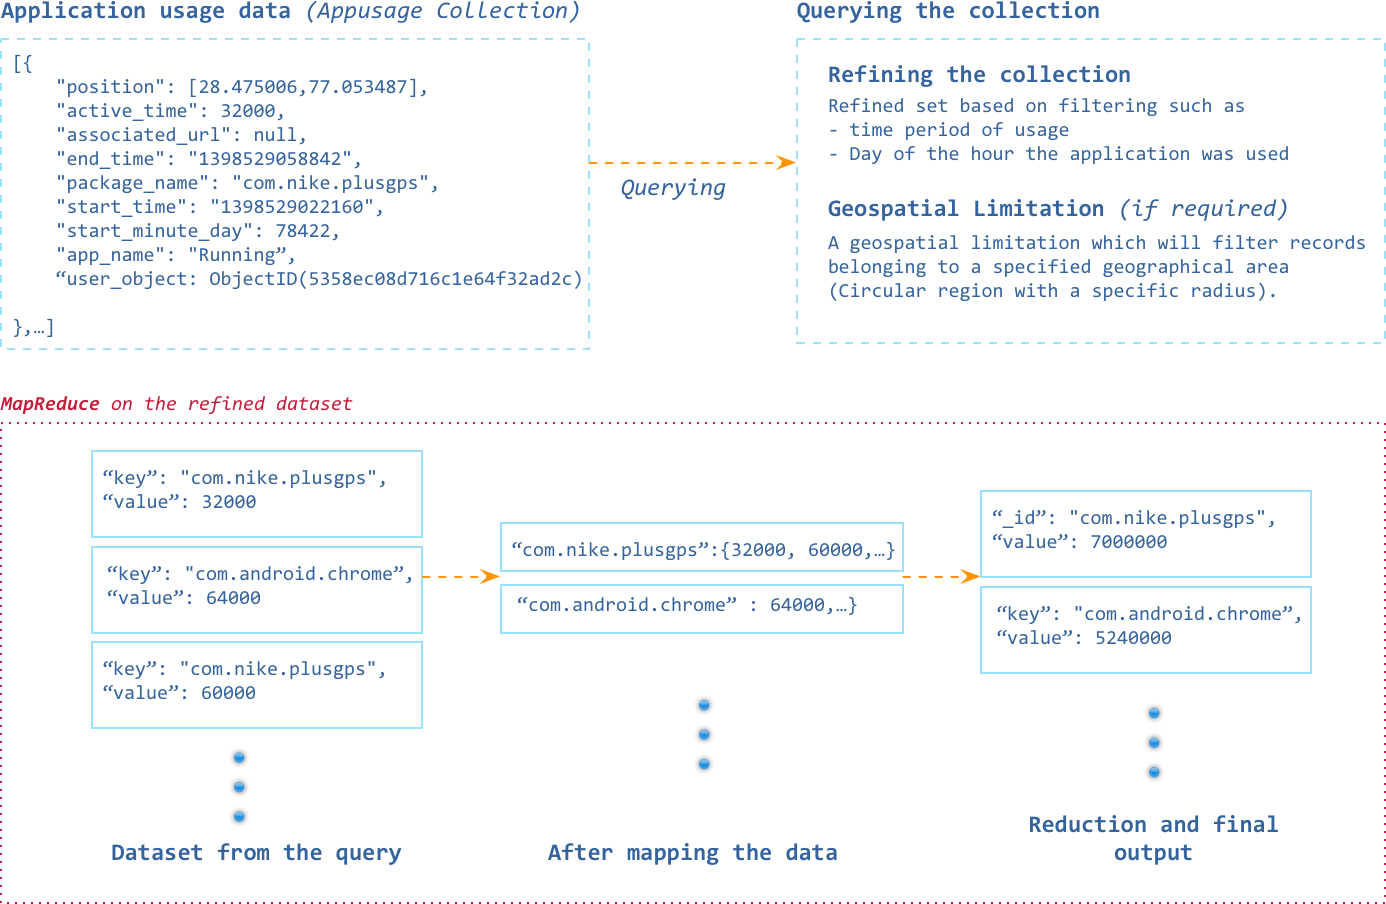
\includegraphics[width=150mm]{MapReduce.png}
  \caption[Applying MapReduce on the app usage data.]{Applying MapReduce on the app usage data.}
 \label{figure:MapReduce}
\end{figure}


The process for extraction of information usually involves aggregating the app usage for each package, however,this can also accommodate filtering based on parameters such as like duration and location information. Location filtering uses the geospatial functions that is provided by mongoDB to reduce the records to a particular area only. The radius along with things such as packages to ignore can all be configured in the config file for the server allowing dynamic changes to the server. The diagram above shows in depth the working of the functionality.

\section{Shortcomings and possible improvements}
\label{AndroidShortcoming}
The application and the framework were both developed over a period of 1.5 months. The purpose of this project was to lay an initial foundation for a robust data gathering application along with a framework which would be re-useable component for context extraction both of which can be re-shaped and used for studies beyond the scope of the present project. This being said, there are various improvements that can be done in the existing application and its web counterpart.

\subsection{Android app}

The android application has a few shortcomings in this first release which can be improved in the future releases along with addition of new features. 

\begin{itemize}

\item Firstly, any improvements that were mentioned in relation to the framework (see section \ref{contextShortcomings}) would effect the overall performance of the app, both in terms of resource consumption and the amount of data that can be gathered using the application.

\item The application at present fails in monitoring web usage if they not performed on the default browser which is accessible by the Browser data provider (\textit{Chrome} on Android 4.0 and above) in the Android SDK. This can effect the overall demographics of the web usage data being collected as interest of the users using other applications to browse internet would not be registered by the application.

\item The application also fails at monitoring tasks which can perform their functionality in the background while user is either using some other application or has switched off the device's screen for example applications such as music players and radios can play audio for the user while running in the background without having the front-end open.

\item The application presently provides analytics and trends information which is very generic which can be customised and converted to a personalised recommendation system among various other possible improvements that can be done to provide more value to the user as an utility application (see section \ref{RecommendationSystem}).
\end{itemize}

\subsection{Web component}

The web component can be improved considerably by adding more features in addition to improving overall performance and scalability of the system.

\begin{itemize}

\item The web component at present does not deal much with the context information, it simply makes use of app usage and location information to provide various results. Future features can make use of all the available information both for research purposes and also for implementing in the application. 

\item The web component's security can be improved by using \textit{Bcrypt}\footnote{Bcrypt: Bowlfish file encryption — http://bcrypt.sourceforge.net/} to store and encrypt private information. Additionally, more precautions can be taken by disassociating the contextual data from the user (see section \ref{UserPrivacy}).

\item The database connection at present picks a connection from the connection pool of the driver, which is a reusable pool of already active connection helping in reducing frequency of opening and closing of connections \cite{MongoLab2013}. There are several things that can be done to improve the speed network transactions.
    \begin{itemize}
        \item Sharding\footnote{MongoDB Sharding - http://docs.mongodb.org/manual/sharding/} maybe applied and to the MongoDB instance to improve the performance of the application and handle increase in the data needs.
        \item At present whenever there is an API call the web service triggers the MongoDB driver along with its customised query which reads data from the database, process it and returns it back to the service to be delivered further to the device. Considering the number of records being created by the devices, once this application has become widespread this process would start taking more and more time to process the request. A caching layer which would store the information in memory instead of reading raw information from the database and processing it again can improve the performance of the queries. Technologies which are meant to handle rapidly changing content in the memory such as Redis\footnote{Redis: An Open source key-value datastore - http://redis.io/} can be used for this purpose in the future.
        
       \item Use of MapReduce technique to perform various complex functions in the application benefits the overall performance, but at present each time the service is called the MapReduce process is performed. This can be avoided by using incremental MapReduce\footnote{MongoDB: Incremental MapReduce - http://docs.mongodb.org/manual/tutorial/perform-incremental-map-reduce/} which automatically reduces the information when new information is added incrementally hence reducing the load on the server by a considerable amount. Future implementations can also look into a Hadoop based MapReduce implementation on the existing MongoDB instance as it has shown promising results \cite{dede2013performance}.
    \end{itemize}

\end{itemize}



\chapter{Putting the collected information to use}
\label{futureUser}
The primary purpose of this stage of the experiment is to design an effective method to gather information from the user on a large scale along with an effective delivery method to do so. The information being gathered is presently stored and and basic feature extraction techniques are being used to provide analytics and trends within the community and in a certain geographical area. However considering the diversity and richness of the data that is and will be available as a result of this application can provide useful input to serval interesting areas of research and help develop various practical applications.

Let us look at a few possible novel approaches to put the information to use in the future.

\section{Intuitive Application Launcher}

A very simple application on the lines of the FALCON system \cite{yan2012fast} which we are already working on would be to build an intuitive launcher for Android devices based on the predictions that would be derived from the gathered information. However, rather then actually launching the application we can provide a much more simplified approach by not pushing the user to make a choice and saving considerable amount of resources.

\begin{figure}[htbp]
 \centering
 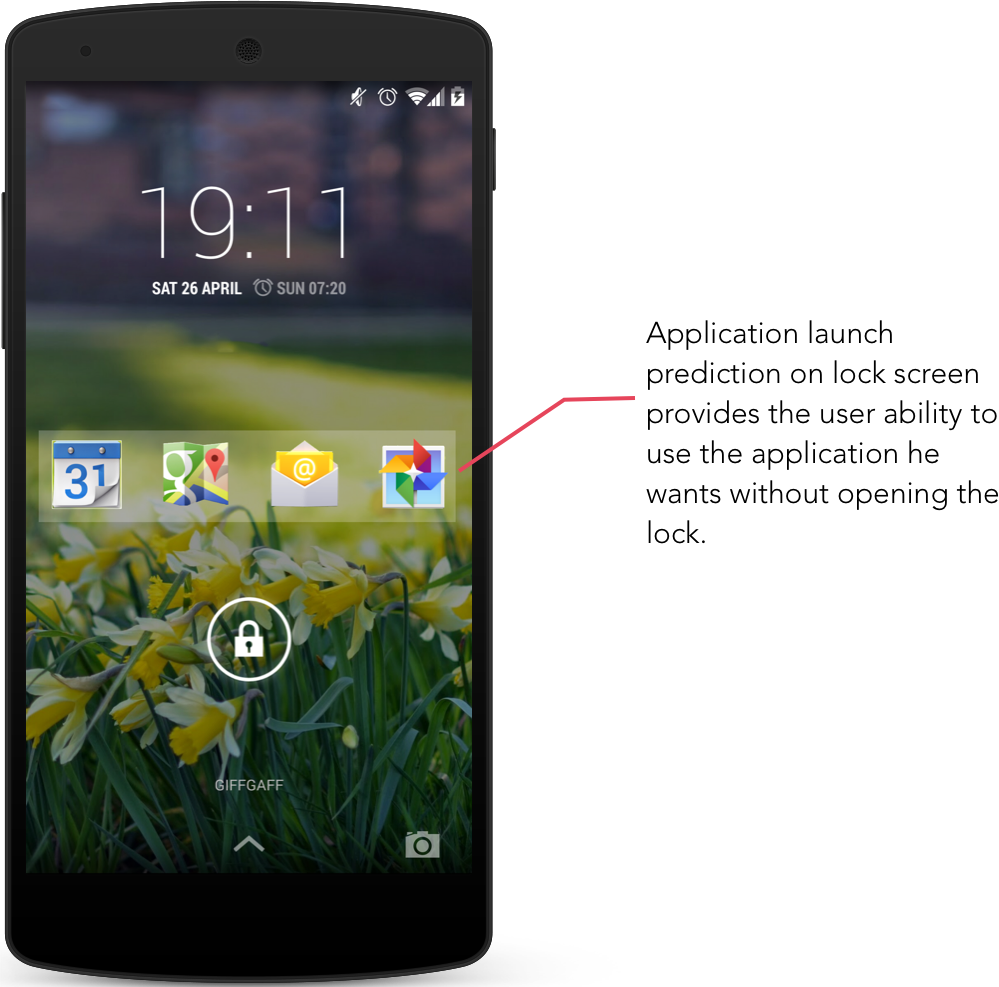
\includegraphics[width=70mm]{IntLauncher.png}
  \caption[An interface prototype for an intuitive application launcher.]{An interface prototype for an intuitive application launcher on the lock screen.}
 \label{figure:SensorInformation}
\end{figure}

Mobile devices usually turn their screens off if there is no activity from the user. Whenever user has to use the device the screen has to switched on and the lock has to be opened. In the event of the screen being switched on, the application which would be integrated with the device's lock screen would present the user with options to launch certain applications. The list of application for the user to choose from would be modified based on time and location. This kind of predictive computing can be very helpful for the user and can prove to make the user's smartphone usage more efficient.

We already have contextual information about the user along with his application usage pattern which we can associate to extract a possible list of application he might want to use. An effective development method with the processing divided between the device and the server would be required to make sure the list can be provided without internet connectivity.

Additionally, the application can learn and improvise itself based on the choices the user makes on the launch screen, i.e., whether or not user selects an application from the list that was provided hence making the application better at predicting application selection over time.

\section{Recommendation system}
\label{RecommendationSystem}

The present version of the application provides recommendation in the form of \textit{What's Trending} using the information that is available about the user's app usage and the location context. The recommendations however are very generic in nature, i.e., recommendations on the basis of the user-base or geographical area. There can be several improvements to the existing features. The system could recommend users what is trending based on their mobile usage pattern, for example if a person uses a certain application for ordering food frequently and there is another application which is popular in the geographical region the application can make a suggestion to him to try out the other application. The prediction can also be influenced by other information that we have collected like gender and user's employment type.

A similar feature can also be developed for the web usage. A recommended reading list can be compiled based on the user's reading habits and the present trends. To achieve this in practicality would require natural language processing to analyse the content of the webpages to understand the relevance of the link. The application would have to understand the user's web usage pattern and derive a web profile for the user and improving it over a period of time based on user's choices and web usage. The content which is recommended is already popular among people the possibility of a favourable recommendation is more likely. This would be similar to the idea presented in \cite{BalabanovicAWP1997} but would be for mobile devices; which would help the system to learn and adapt faster.


\section{Content and application pre-caching}

Information gathered about content being accessed on the web or application being launched alongside the location context provides us an insight about what is popular in a particular geographical region. This as discussed earlier can be personalised to provide what user tends to view or use at a particular location frequently. Application can be launched and kept running in the background as to reduce the wait time for the user when the application is launched and possibly loading itself into the memory or maybe loading content from the web.


In relation to the web, this information can be used in a very different scenario. With the knowledge about localised trends on the web an interface can be created which can be made accessible externally to provide possible websites people might use at a particular location. This information can then be linked with the local cellular network or WiFi access points and the content can be cached on the network itself provided improved loading time for the users of the network hence improving the overall user experience. This can be further improvised further by anticipating and then caching possible future navigation from the current website reducing the loading time of requests even further beyond what is achievable using the trends information \cite{cheluvaraju2011anticipatory}.

\chapter{Performance evaluation}
\label{PeformanceEval}

In this section we presents the various statistics, results and observations obtained by running \textit{WebSense} on 3 different android devices for 2 consecutive days. The information was stored on the server and processed and provided back to the device showcase on the user interface. We look into the various parameters that govern the performance of the application and the server component and then we also try to analyse the results and try to find the possible reasons and improvements that can be done based on it.


\section{Application \& framework performance}

The performance of an application the framework is benchmarked based on various factors. The hardware itself plays a very vital role in the process. In order to better understand the performance on a much broader scale we use 3 different devices for 2 days in an experiment conducted over 6 days. During this duration the devices were constantly taken out and used as personal devices providing us results for normal mobile usage.

The devices that were chosen were, LG Nexus 5, LG Nexus 4 and Samsung Galaxy S5. All of them running Android version 4.4.2. The specifications of the devices are as follows.

\begin{itemize}
\item \textbf{LG Nexus 4}
    \begin{itemize}
        \item 1.5 GHz quad-core Snapdragon S4 Pro processor
        \item 2 GB RAM
        \item 2100 mAh battery
        \item 16 GB Internal storage
    \end{itemize}

\item \textbf{LG Nexus 5}
    \begin{itemize}
        \item 2.26 GHz quad-core Snapdragon 800 processor
        \item 2 GB RAM
        \item 2300 mAh battery
        \item 16 GB Internal storage
    \end{itemize}

\item \textbf{Samsung Galaxy S4}
    \begin{itemize}
        \item  Snapdragon 600 (quad-core 1.9 GHz Krait 300 CPU \& Adreno 320 GPU)
        \item 2 GB RAM
        \item 3600 mAh battery
        \item 32 GB Internal storage
    \end{itemize}

\end{itemize}

Having multiple devices helps us in averaging out the performance and helps in detecting platform specific anomalies in the system. Firstly let us look into the stability of the application, using ACRA we are able to analyse crashes and issues faced on the device without being connected to the development machine, it catches crashes that happen in the background thread as well. Over the duration of 6 days the server received 1 crash report which when analysed and attributed to concurrent writes being performed onto the preferences causing a deadlock on a rare occasion. Apart from the crash-logs, we can also analyse the stability of the application by analysing the uptime in the settings application present in the OS which allows us to see the uptime of background services. On the Nexus 5 device each of the services had an uptime of over 90 hours, well over the experiment period. Similar observations were made on Nexus 4 and S5 as well. This verifies the application and the framework can provide an near 100\% uptime in monitoring user's actions.

Let us look into memory foot-print of the application. The app constantly keeps alive 3 services to monitor and synchronise information, even if the operating system destroys the services in case of low memory \cite{AndroidAppLifeCycle} the service's self reviving cycle brings it at back as soon as possible (See appendix \ref{AppConstants} for revival time). The application does not require a front end for monitoring so it there is no constant front-end memory footprint. Using Android's DDMS \cite{AndroidDDMS} and an additional app called Memory Usage\footnote{https://play.google.com/store/apps/details?id=mem.usage}, the memory usage of the application was analysed to vary between 16MB to 24MB. The peak in the usage when the application has the front end active and is performing web requests to fetch data. It has a similar footprint across all the devices.

The next crucial aspect is power consumption; the power consumption various with the various settings of the application, for the present configuration (See appendix \ref{Config}). The application consumed 4\%, 6\% and 7\% battery on Nexus 5, Nexus 4 and Galaxy S4 during the experimental cycle.

In terms of data bandwidth usage, the application has shown to have a very low requirement. The web requests being made are all GZIP compression enabled which allows to reduce the call footprint drastically for the provided batch. In addition to save the information the system makes use of WiFi over data connections, which too is governed by the configuration factor (See appendix \ref{Config}).

The application transferred over 1350 KB of data over WiFi on an average and only 120 KB on cellular data. However, this statistics is highly variant as it depends on availability of WiFi and the mobility of the user.

Overall, from the evaluation of the application we have learnt of a few new issues in the application, areas that we can look into like reduction of the memory footprint. In addition to this more detailed test related to power consumption need to be conducted on various configurations in order to tweak and improve the overall performance of the application.

\section{Web application performance}

The web application is built on Node.js with MongoDB as its database. The server is an Amazon EC2 instance with 0.613GB of RAM and other similar variable low end specs. We analyse the performance of requests which constitutes of mechanisms such as Geospatial requests and MapReduce in place; processing of the data over a set of 8580 records of application usage and 7362 records for context information (integrated at a later stage).

Over its short duration of being operational the web component has already scrapped information about 78 android apps and 33 websites consisting of image URLs, ratings, description, category , etc.

Over the duration of the experiment on three devices combined there were 2477 records created on the server with an astonishing 33.28 hours of phone activity, resulting in an average of ~45 seconds per activity (Please consider that change in contextual information is considered as a different activity).

\begin{table}[htdp]

\begin{center}
\begin{tabularx}{\textwidth}{ XXX }
 
  \begin{center}\textbf{API end point}\end{center} & \begin{center}\textbf{Response Time}\end{center} \\
   \hline
  /app/trends/monthly  & 199ms  \\
  /app/trends/weekly   & 113ms  \\
  /app/trends/daily   &  45ms    \\ 
  /web/trends/monthly  & 27ms  \\
  /web/trends/weekly   & 22ms  \\
  /web/trends/daily   &  11ms    \\ 
    /app/nearby/monthly  & 109ms  \\
  /app/nearby/weekly   & 75ms  \\
  /app/nearby/daily   &  35ms    \\ 
   \hline
  \end{tabularx}

\end{center}
\caption{Response time for API end points.}
\label{timingcomparison}
\end{table}%

Table \ref{timingcomparison} highlights the request response time of the various request that can be made. It is vital to note that the time required to process request relies on the number of records that it has to process and the network speed. So when new users are added and the number of records increase which would have effects on the response time as well, hence a more powerful server would be required to handle such requests. We will further discuss how do handle such situations and improve performance in chapter \ref{challenges}.

When the data was further analysed it was inferred that more then 40\% of the contextual records for S4 were for WiFi information, although this can be useful but with several repetitions, it can be improved and made efficient. An approximate of 11\% contextual records and 18\% of application usage data lacked location information which can be attributed to several factors such as unable to get a fix on GPS, provider being turned off, all the more reason to further investigated into the location obtaining process. All this presents us with room for improvement in the framework and the application as well.

\chapter{Challenges and concerns}
\label{challenges}

As with any research, there are several challenging aspects and concerns surrounding this project that are to be considered both in terms of the present scope of the application/framework and in terms of the future prospects where the research can be used. In this chapter we briefly look into some of the key challenges faced by this project.

\section{Platform restrictions and application deployment}
\label{PlatformDeployment}
The framework and the application in this report were both developed to be used on the Android operating system, this restricts the user who can participate in the study to only the one's with a smartphone which runs Android OS; users with other devices cannot contribute to the study in any way. This not only can cause an overall decrease in the number of participants, it can also effect the demographics and the quality of the data being collected as there can indeed be a variation in smartphone usage based on the operating system. Even though research \cite{gartnerMobileSurvey2013} shows that Android holds a majority among the masses in terms of mobile marketshare, there are still a considerable number of users using other operating systems moreover the demographics of operating system usage can very widely across geographies. This presents a very serious concern and also a possible direction to look into in the future research as it is being faced by other researchers involved in similar crowd-sensing experiments \cite{balan2011real}. 

It should also be taken into consideration that Android is a very flexible platform which lets us build applications which can access such a wide array of information, some of which is currently not possible on other operating systems such as iOS. iOS, for example is governed by a sandbox policy \cite{AppleiOSPolicy} which does not allow to application to access information beyond its assigned limit (such as extracting information about the running applications).

Being a crowd-sourcing application, the application is to be installed from an application store for android which presents yet another problem. This puts the decision of participation in the study solely on the fact that the user recognises the application on the store, installs and retains it on his device. The participation rate would vary depending on the application's popularity and would take some time to provide a considerable dataset which is explained further in \cite{xiao2013lowering}, it also recommends on how to remove installation of the application from the critical path but is presently not possible on Android for the type of information we require.

\section{Resource utilisation}

The purpose of the application is to monitor the how the user interacts with the smartphone and to observe the various contexts and sensors, which means that it has to quasi-continuously execute series of scans and poll sensors/API's in order to extract the required information. The extracted information has to be then stored on the disk and also has to be sent to the web server frequently for analysis using the internet connection of the device. All of these processes require a considerable amount of processing power, battery power and internet bandwidth (which in-turn means that the user may incur some monitory expense), hence making this a very critical aspect of the application which would have to be optimised.

For the application to be able to gather realistic information from the user it requires to be able to do it in an ubiquitous way, which would not be possible if the application is consuming too much of resources hence causing reduction in the average battery cycle of the smartphone or reducing the data bandwidth available to other apps which would make the connectivity an issue for other applications and causing the user experience of the applications to deteriorate. 

Making the application perform all the required tasks while being efficient enough to have a very minimal footprint on the device was one of the key challenges of the project. Various steps were taken during development to make sure that the resource utilisation is kept to a minimum (see chapter \ref{PeformanceEval} for detailed evaluation). For example, the application has an optimised synchronisation process, it prefers synchronisation of records on a WiFi connection rather then a cellular data connection, however if a threshold is reached in the collected information it tries to synchronise on cellular data network to reduce changes of data loss. The polling tasks of the framework are programmed to be functioned at fixed intervals which are specific to tasks and has a direct correlation with the type of information it provides, power consumption and required level of freshness of the information.The overall polling of context is done by the framework at certain fixed intervals each reflecting on the power consumption and the requirement for freshness of the data.

The resource utilisation can further be improved by developing the framework to perform adaptive sensing instead of scanning at fixed intervals. We can also do some pre-processing on the data (e.g., remove non required elements) hence reducing the overall bandwidth usage of the application. Deriving a relation between sensing rate and the power level of the device can help improve the battery life of the device. Sources of information which consume lesser power should be given preference for example using network instead of GPS for location detection is proven to save resources with an acceptable location accuracy \cite{zhuang2010improving}.

\section{Data privacy}
\label{UserPrivacy}
One of the most common and possibly the most serious concern while developing a system that deals with user's personal information is privacy. Some argue that it is the system developer's responsibility to take into consideration the privacy of the user and his information while designing the system \cite{adams2001privacy}. However it is essential to understand privacy concerns in these systems does not just end at ensuring restricted and authorised access of information through secure channels, there are several other technical and ethical aspects to it.

The application collects considerable amount of information about the end-user and stores it remotely, which allows a possibility for any external person to profile the user based on the information provided by third party which the user might not permit if asked for. It is not compulsory that the records have to be linked to the user for the breach to occur; inferences can be derived by using contextual information that is available along with external information sources to identify events and user activities \cite{minch2004privacy}. Hence, keeping the information secure and impossible to use for identification from preying hands is very essential.

The first step which several usability studies mention in relation to such system's privacy aspect is to be transparent about the process that the application follows. Taking the user's consent and providing proper explanation about the reason for the collection of each and every contextual information from the user \cite{SymmKK2006,picard2002computers}; providing an insight on the data that is being collected and the subsequent use it would be put to allows the end-user to take a stand on whether or not he wishes to continue supplying data.

The possible use of the data gathered about user's activities, context and patterns can be to recommend information to the user in the future (see section \ref{RecommendationSystem}). This may result in causing a subliminal behaviour changes which can very well be the purpose of the application as further demonstrated in various app mentioned in \cite{lathia2013smartphones} however it can also be a repercussion of the app and may also cause a negative implication (for example, the application may recommend the user entertainment/social networking application while he is working based on his overall usage trends hence interrupting him and causing distraction). The control of how recommendations are provided or even how the application would be effecting the user's behaviour should hence be in the hands of the user and not the developer. In addition to this the application should also provide the user the ability to discontinue monitoring whenever he wants, which is taken care of in the form of a logout option in the application which terminates all monitoring tasks.

\chapter{Related Work}
Over the last few years there have been several efforts in the form of researches that have worked on creating an extensible context sensing framework on various mobile platforms. Similarly there have been experiments conducted to gather information about user's smartphone usage and analyse mobile demographics in a general sense. In this chapter we shall briefly look into some of the more interesting and promising research work so far.

One of the most extensive work that has been done in the field of sensing on the mobile platform is the EmotionSense project\footnote{EmotionSense — http://emotionsense.org/}. The application is a part of a research whose goal was building a framework for mobile to assist in studies about user's emotions and behaviour. Previously developed for Nokia Symbian 60 platform \cite{rachuri2010emotionsense}, EmotionSense now has been re-modelled to work for the Android platform, several components of which have been open-sourced. There are several interesting components of the system which makes it very promising to use in any large scale mobile sensing project. The EmotionSense system constitutes of several sensor monitors which are of both polling and broadcast receiver model in nature. The inference engine present in the system provides the system the ability to adapt itself based on circumstances; for example monitoring of location only needs to happen when the user is moving \cite{rachuri2010emotionsense}. The sensor information is then stored in a knowledge base. In addition to this the framework (Symbian 60 version) also provides functionality for speaker and emotion recognition. However the android version presently provides only adaptive sensing and lacks methods for extraction of contextual information that are available on the more modern version of the operating system. Several researches which have made use of the framework have tried to extend it further and used it to build systems that can perform features like speaker recognition \cite{lathia2013smartphones}.

Another example for a sensing framework is the Mobile Sensing Framework (MSF) described in \cite{novakextensible2013}. The framework is designed for Android and makes use of Ambient Dynamics \cite{carlson2012dynamix} which enables it to dynamically adapt and control sensing after installation. The framework also enables to mine and extract historical context which can be used in various ways. \textit{funf open sensing framework}\footnote{http://www.funf.org} provides feature similar to MSF, however instead of letting user choose the way to store information the framework provides an inbuilt integration with Dropbox\footnote{http://www.dropbox.com/} for automatically saving the information.

In terms of tracking and understanding user application usage there have been several studies and applications. One of the most promising one is FALCON \cite{yan2012fast}, a predictive app launching system which integrates with the Windows mobile operating system. Like \textit{WebSense}, the application accesses mobile usage patterns of the user and combines it with location and other contextual parameters to predictively launch applications. The framework also takes into consideration the power, memory, launch time, energy and bandwidth factors prior launching the application and improves itself over the time \cite{yan2012fast}.

Another experiment \cite{do2010their}. Focused on building a framework to collect and mine large-scale patterns in mobile usage data presents various interesting patterns and statistics about mobile usage of a normal user for example it shows that user's tend to use majorly system application, primarily calling and SMS (which might be different in the past few years with new communication technologies). It also shows behaviour patterns among users and how several applications and why people interacts with it, are interrelated.

\chapter{Future Work and conclusion}
The application and the framework lays a foundation for a much more complex and useful anticipatory system through which not only can we understand more about the users but also help design future technologies to improve their experiences on mobile devices. Throughout this report we have discussed the various issues, shortcomings and have pointed out the scope for improvements in the present system. The framework presents us with a very simple yet effective approach to gather contextual data from smartphones of the user with the minimal development efforts for integration; providing the developers with much more time to concentrate on the real problem at hand rather then being concerned about data gathering and its efficiency. The contextual information that is being provided by the framework can be further improved both in terms of the quality and the details it can provide. Various other contextual sources can also be considered along with various other improvements that we have discussed in the section \ref{contextShortcomings} in the future version of the framework along with some serious thoughts on the observations that we have made in chapter \ref{PeformanceEval}.

The android application which is at its initial stages of development, presently is extracting contextual information with the help of the framework and working alongside various other system components; however the data is at present being used for basic predictions tasks and application/web recommendations. As we have seen in section \ref{contextShortcomings} the application would also require improvements both in terms of sensing techniques and in terms of the quality of information it provides us, information which could be harnessed to build systems and conduct further research;all of which shows us the potential of this application and the framework.

Mobile presence is not only a lifestyle anymore it has become a necessity, helping us in performing our day to day task and constantly helping us simplify our lives. It has already achieved a near-ubiquitous presence by blending itself into our lives and create an impact on it which we take for granted everyday. This has provided us an avenue for research in the forms of device capable of sensing information which was previously not possible without interrupting the user. Understanding how the user behaves and its relation to the context that surrounds him provides us an insight in creating a model for user's smartphone usage. This information empowers us in creating systems which can assist the user, help him make better choices or make him recommendations and even more bold and challenging ideas to create a better user experience in the future.
 
\bibliographystyle{chicago}
\bibliography{mini_project_report}

%APPENDICES
\appendix
%Mini-project declaration
%\clearpage
\chapter{Mini-Project Declaration}
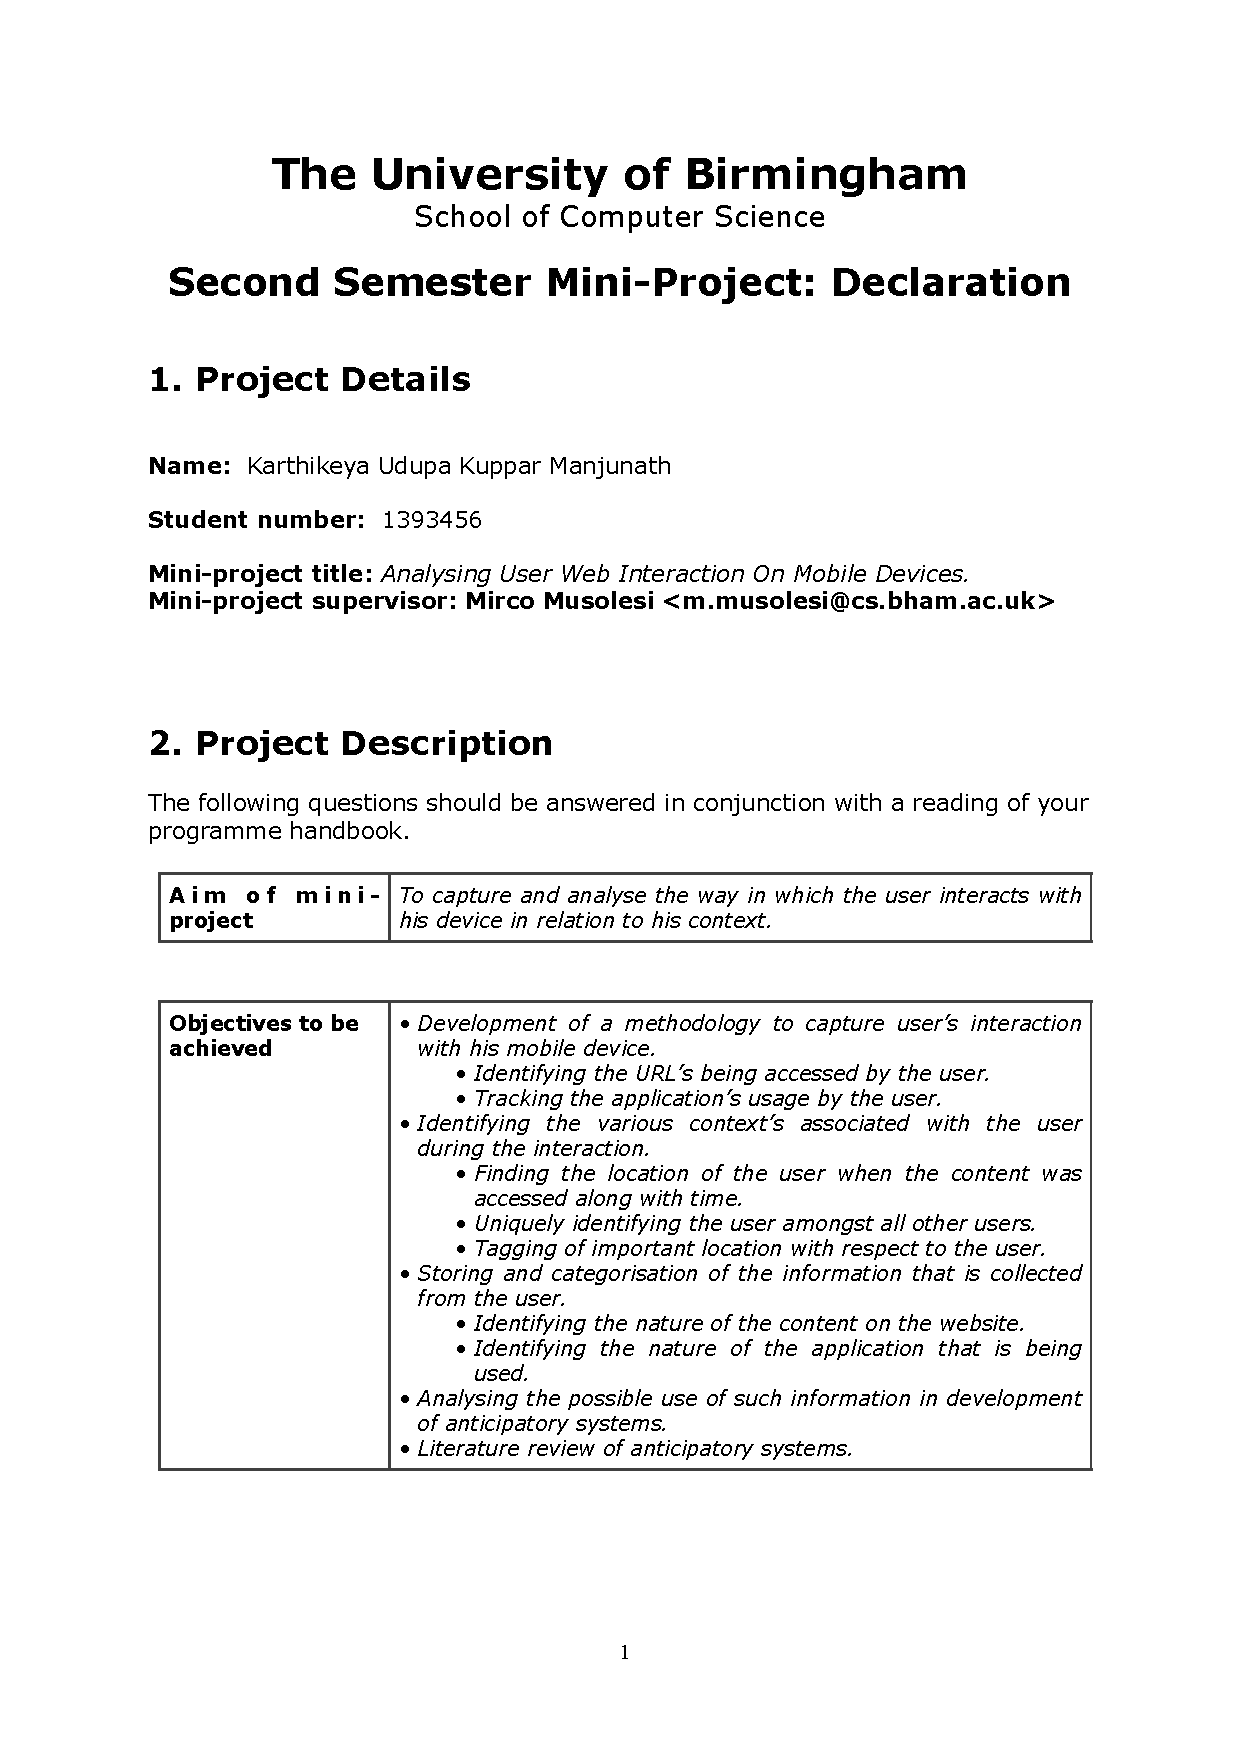
\includepdf[pages={1,2}]{Declaration.pdf}

\chapter{Statement of information search strategy}
\section{Parameters for literature search}
\textit{Forms of literature}: The following literature sources were reviewed:
\begin{itemize}
\item Conference papers
\item Journal articles
\item Theses
\item Books
\item API Documentation
\end{itemize}

\textit{Geographical/language coverage}: Reference papers used for this work is were from North America and Western Europe. Preferred language for all the reference paper was English.
\section{Appropriate search tools}
\begin{itemize}
\item \textit{Google Scholar}: 
Was used to retrieve conference papers, journal articles and some theses. This search engine was used for a wide coverage of research topics and experiments conducted in the area of anticipatory computing, context sensing, user behaviour monitoring among others.
\item \textit{Android SDK Documentation}: The android SDK was used to understand the operating system's functioning and its various components.
\end{itemize}


\chapter{Configurations}
\label{Config}
\begin{program}
  \begin{verbatim}
public static long BG_SERVICE_ALARM_RELOAD_TIME = 25*1000L; //service revival time.
public static long TASK_POLLER_TIMER = 4*1000L;
public static int MIN_RECORD_FOR_SYNC = 20; //for WiFi
public static int RECORD_THRESHOLD_FOR_FORCED_SYNCED = 100; //on cellular.
public static int RECORD_BATCH_COUNT = 50;
	
\end{verbatim}
\caption{Constants for the \textit{WebSense} application.}
\label{AppConstants}
\end{program}

\begin{program}
  \begin{verbatim}
mContextManager.monitorContext(
ContextManagerServices.CTX_FRAMEWORK_LOCATION, 60*60*1000L);			mContextManager.monitorContext(
ContextManagerServices.CTX_FRAMEWORK_BATTERY, 10*60*1000L);
mContextManager.monitorContext(
ContextManagerServices.CTX_FRAMEWORK_WIFI, 30*60*1000L);
mContextManager.monitorContext(
ContextManagerServices.CTX_FRAMEWORK_SIGNALS, 15*60*1000L);
mContextManager.monitorContext(
ContextManagerServices.CTX_FRAMEWORK_EVENTS, 2*60*1000L);
mContextManager.monitorContext(
ContextManagerServices.CTX_FRAMEWORK_BLUETOOTH, 10*60*1000L);
			
	
\end{verbatim}
\caption{Initialisation for sensing from \textit{WebSense} with minimum broadcast timing specified.}
\label{ContextInitCalls}
\end{program}

\begin{program}
  \begin{verbatim}

public static String DEFAULT_LOCATION_PROVIDER = NETWORK_PROVIDER;
public static long MAXIMUM_ACCEPTABLE_TIME = 40*1000L;
public static long MAXIMUM_ACCEPTABLE_DISTANCE = 0;
public static long SHORT_POLLING_INTERVAL =  15*60*1000L; 
public static final long MINUTE_POLLING_INTERVAL = 3*60*1000L;
public static final long LONG_POLLING_INTERVAL = 30*60*1000L;
public static final long GRANULAR_POLLING_INTERVAL = 10*1000L;
		
\end{verbatim}
\caption{Constants for the Android context sensing framework.}
\label{ContextFrameworkConstants}
\end{program}



	
\end{document}